\documentclass[twoside]{book}

% Packages required by doxygen
\usepackage{calc}
\usepackage{doxygen}
\usepackage{graphicx}
\usepackage[utf8]{inputenc}
\usepackage{makeidx}
\usepackage{multicol}
\usepackage{multirow}
\usepackage{textcomp}
\usepackage[table]{xcolor}

% Font selection
\usepackage[T1]{fontenc}
\usepackage{mathptmx}
\usepackage[scaled=.90]{helvet}
\usepackage{courier}
\usepackage{amssymb}
\usepackage{sectsty}
\renewcommand{\familydefault}{\sfdefault}
\allsectionsfont{%
  \fontseries{bc}\selectfont%
  \color{darkgray}%
}
\renewcommand{\DoxyLabelFont}{%
  \fontseries{bc}\selectfont%
  \color{darkgray}%
}

% Page & text layout
\usepackage{geometry}
\geometry{%
  a4paper,%
  top=2.5cm,%
  bottom=2.5cm,%
  left=2.5cm,%
  right=2.5cm%
}
\tolerance=750
\hfuzz=15pt
\hbadness=750
\setlength{\emergencystretch}{15pt}
\setlength{\parindent}{0cm}
\setlength{\parskip}{0.2cm}
\makeatletter
\renewcommand{\paragraph}{%
  \@startsection{paragraph}{4}{0ex}{-1.0ex}{1.0ex}{%
    \normalfont\normalsize\bfseries\SS@parafont%
  }%
}
\renewcommand{\subparagraph}{%
  \@startsection{subparagraph}{5}{0ex}{-1.0ex}{1.0ex}{%
    \normalfont\normalsize\bfseries\SS@subparafont%
  }%
}
\makeatother

% Headers & footers
\usepackage{fancyhdr}
\pagestyle{fancyplain}
\fancyhead[LE]{\fancyplain{}{\bfseries\thepage}}
\fancyhead[CE]{\fancyplain{}{}}
\fancyhead[RE]{\fancyplain{}{\bfseries\leftmark}}
\fancyhead[LO]{\fancyplain{}{\bfseries\rightmark}}
\fancyhead[CO]{\fancyplain{}{}}
\fancyhead[RO]{\fancyplain{}{\bfseries\thepage}}
\fancyfoot[LE]{\fancyplain{}{}}
\fancyfoot[CE]{\fancyplain{}{}}
\fancyfoot[RE]{\fancyplain{}{\bfseries\scriptsize Generated on Mon Jun 27 2016 02\-:49\-:48 for Sigma  $\vert$  A\-P\-I by Doxygen }}
\fancyfoot[LO]{\fancyplain{}{\bfseries\scriptsize Generated on Mon Jun 27 2016 02\-:49\-:48 for Sigma  $\vert$  A\-P\-I by Doxygen }}
\fancyfoot[CO]{\fancyplain{}{}}
\fancyfoot[RO]{\fancyplain{}{}}
\renewcommand{\footrulewidth}{0.4pt}
\renewcommand{\chaptermark}[1]{%
  \markboth{#1}{}%
}
\renewcommand{\sectionmark}[1]{%
  \markright{\thesection\ #1}%
}

% Indices & bibliography
\usepackage{natbib}
\usepackage[titles]{tocloft}
\setcounter{tocdepth}{3}
\setcounter{secnumdepth}{5}
\makeindex

% Hyperlinks (required, but should be loaded last)
\usepackage{ifpdf}
\ifpdf
  \usepackage[pdftex,pagebackref=true]{hyperref}
\else
  \usepackage[ps2pdf,pagebackref=true]{hyperref}
\fi
\hypersetup{%
  colorlinks=true,%
  linkcolor=blue,%
  citecolor=blue,%
  unicode%
}

% Custom commands
\newcommand{\clearemptydoublepage}{%
  \newpage{\pagestyle{empty}\cleardoublepage}%
}


%===== C O N T E N T S =====

\begin{document}

% Titlepage & ToC
\hypersetup{pageanchor=false}
\pagenumbering{roman}
\begin{titlepage}
\vspace*{7cm}
\begin{center}%
{\Large Sigma $\vert$ A\-P\-I \\[1ex]\large Version 0.\-0.\-1 }\\
\vspace*{1cm}
{\large Generated by Doxygen 1.8.6}\\
\vspace*{0.5cm}
{\small Mon Jun 27 2016 02:49:48}\\
\end{center}
\end{titlepage}
\clearemptydoublepage
\tableofcontents
\clearemptydoublepage
\pagenumbering{arabic}
\hypersetup{pageanchor=true}

%--- Begin generated contents ---
\chapter{Sigma C++ Documentation}
\label{index}\hypertarget{index}{}T\-O\-D\-O\-:

The source code can be found here\-: \href{https://github.com/DavidSaxon/Sigma}{\tt https\-://github.\-com/\-David\-Saxon/\-Sigma} 
\chapter{Namespace Index}
\section{Namespace List}
Here is a list of all documented namespaces with brief descriptions\-:\begin{DoxyCompactList}
\item\contentsline{section}{\hyperlink{namespacesigma}{sigma} \\*Global namespace which contains all built-\/in aspects of Sigma }{\pageref{namespacesigma}}{}
\item\contentsline{section}{\hyperlink{namespacesigma_1_1core}{sigma\-::core} \\*The core backend A\-P\-I of Sigma. Sigma core is entirely detached from any Sigma U\-I }{\pageref{namespacesigma_1_1core}}{}
\item\contentsline{section}{\hyperlink{namespacesigma_1_1core_1_1tasks}{sigma\-::core\-::tasks} \\*The task management A\-P\-I module of Sigma }{\pageref{namespacesigma_1_1core_1_1tasks}}{}
\end{DoxyCompactList}

\chapter{Hierarchical Index}
\section{Class Hierarchy}
This inheritance list is sorted roughly, but not completely, alphabetically\-:\begin{DoxyCompactList}
\item \contentsline{section}{sigma\-:\-:core\-:\-:Callback\-Handler$<$ function\-\_\-parameters $>$}{\pageref{classsigma_1_1core_1_1_callback_handler}}{}
\item Callback\-Interface\-Base\begin{DoxyCompactList}
\item \contentsline{section}{sigma\-:\-:core\-:\-:Callback\-Interface$<$ function\-\_\-parameters...$>$}{\pageref{classsigma_1_1core_1_1_callback_interface}}{}
\item \contentsline{section}{sigma\-:\-:core\-:\-:Callback\-Interface$<$ function\-\_\-parameters $>$}{\pageref{classsigma_1_1core_1_1_callback_interface}}{}
\end{DoxyCompactList}
\item \contentsline{section}{sigma\-:\-:core\-:\-:Scoped\-Callback}{\pageref{classsigma_1_1core_1_1_scoped_callback}}{}
\item \contentsline{section}{sigma\-:\-:core\-:\-:tasks\-:\-:Task}{\pageref{classsigma_1_1core_1_1tasks_1_1_task}}{}
\end{DoxyCompactList}

\chapter{Class Index}
\section{Class List}
Here are the classes, structs, unions and interfaces with brief descriptions\+:\begin{DoxyCompactList}
\item\contentsline{section}{\hyperlink{classsigma_1_1core_1_1util_1_1_arc_log_verbosity_v}{sigma\+::core\+::util\+::\+Arc\+Log\+Verbosity\+V} \\*Meta\+Engine Visitor object used to retrieve arclog\+::\+Verbosity values from a metaengine\+::\+Document }{\pageref{classsigma_1_1core_1_1util_1_1_arc_log_verbosity_v}}{}
\item\contentsline{section}{\hyperlink{classsigma_1_1core_1_1_callback_handler}{sigma\+::core\+::\+Callback\+Handler$<$ function\+\_\+parameters $>$} \\*Object used to handle callbacks of a given function type }{\pageref{classsigma_1_1core_1_1_callback_handler}}{}
\item\contentsline{section}{\hyperlink{classsigma_1_1core_1_1_callback_interface}{sigma\+::core\+::\+Callback\+Interface$<$ function\+\_\+parameters $>$} \\*Used to register global, static, and member functions as callbacks }{\pageref{classsigma_1_1core_1_1_callback_interface}}{}
\item\contentsline{section}{\hyperlink{classmeta__qt_1_1_qt_window_flags_v}{meta\+\_\+qt\+::\+Qt\+Window\+Flags\+V} \\*Meta\+Engine Visitor object used to retrieve a bitwise O\+R of Qt\+::\+Window\+Flags }{\pageref{classmeta__qt_1_1_qt_window_flags_v}}{}
\item\contentsline{section}{\hyperlink{classsigma_1_1core_1_1tasks_1_1_root_task}{sigma\+::core\+::tasks\+::\+Root\+Task} \\*T\+O\+D\+O }{\pageref{classsigma_1_1core_1_1tasks_1_1_root_task}}{}
\item\contentsline{section}{\hyperlink{classsigma_1_1core_1_1_scoped_callback}{sigma\+::core\+::\+Scoped\+Callback} \\*Object that holds the id of a callback function and aids in life cycle management of the callback }{\pageref{classsigma_1_1core_1_1_scoped_callback}}{}
\item\contentsline{section}{\hyperlink{classsigma_1_1gui_1_1startup_1_1_splash_screen}{sigma\+::gui\+::startup\+::\+Splash\+Screen} \\*Base widget for the Sigma startup splash screen }{\pageref{classsigma_1_1gui_1_1startup_1_1_splash_screen}}{}
\item\contentsline{section}{\hyperlink{classsigma_1_1core_1_1tasks_1_1_task}{sigma\+::core\+::tasks\+::\+Task} \\*T\+O\+D\+O }{\pageref{classsigma_1_1core_1_1tasks_1_1_task}}{}
\item\contentsline{section}{\hyperlink{classmeta__qt_1_1_widget_position}{meta\+\_\+qt\+::\+Widget\+Position} \\*Meta\+Engine Visitor that is used to retrieve the absolute position of a Q\+Widget as a Q\+Point from a J\+S\+O\+N object type in a metaengine\+::\+Doument }{\pageref{classmeta__qt_1_1_widget_position}}{}
\item\contentsline{section}{\hyperlink{classmeta__qt_1_1_widget_size}{meta\+\_\+qt\+::\+Widget\+Size} \\*Meta\+Engine Visitor that is used to retrieve the absolute size of a Q\+Widget as a Q\+Size from a J\+S\+O\+N object type in a metaengine\+::\+Doument }{\pageref{classmeta__qt_1_1_widget_size}}{}
\end{DoxyCompactList}

\chapter{File Index}
\section{File List}
Here is a list of all documented files with brief descriptions\-:\begin{DoxyCompactList}
\item\contentsline{section}{/home/david/\-Dropbox/\-Development/\-Sigma/\-Sigma/src/cxx/sigma/{\bfseries \-\_\-\-\_\-sigma.\-hpp} }{\pageref{____sigma_8hpp}}{}
\item\contentsline{section}{/home/david/\-Dropbox/\-Development/\-Sigma/\-Sigma/src/cxx/sigma/core/\hyperlink{_callback_8hpp}{Callback.\-hpp} \\*Classes that make up Sigma's callback system }{\pageref{_callback_8hpp}}{}
\item\contentsline{section}{/home/david/\-Dropbox/\-Development/\-Sigma/\-Sigma/src/cxx/sigma/core/\hyperlink{_sigma_8hpp}{Sigma.\-hpp} \\*The main entry point for the Sigma A\-P\-I }{\pageref{_sigma_8hpp}}{}
\item\contentsline{section}{/home/david/\-Dropbox/\-Development/\-Sigma/\-Sigma/src/cxx/sigma/core/tasks/\hyperlink{_root_task_8hpp}{Root\-Task.\-hpp} }{\pageref{_root_task_8hpp}}{}
\item\contentsline{section}{/home/david/\-Dropbox/\-Development/\-Sigma/\-Sigma/src/cxx/sigma/core/tasks/\hyperlink{_task_8hpp}{Task.\-hpp} }{\pageref{_task_8hpp}}{}
\item\contentsline{section}{/home/david/\-Dropbox/\-Development/\-Sigma/\-Sigma/src/cxx/sigma/core/tasks/\hyperlink{_tasks_domain_8hpp}{Tasks\-Domain.\-hpp} \\*Provides the outwards facing entry point for the Task Management A\-P\-I domain }{\pageref{_tasks_domain_8hpp}}{}
\end{DoxyCompactList}

\chapter{Namespace Documentation}
\hypertarget{namespacesigma}{}\section{sigma Namespace Reference}
\label{namespacesigma}\index{sigma@{sigma}}


the global namespace which contains all built-\/in aspects of Sigma.  


\subsection*{Namespaces}
\begin{DoxyCompactItemize}
\item 
 \hyperlink{namespacesigma_1_1core}{core}
\begin{DoxyCompactList}\small\item\em The core backend A\+P\+I of Sigma. Sigma core is entirely detached from any Sigma U\+I. \end{DoxyCompactList}\item 
 \hyperlink{namespacesigma_1_1gui}{gui}
\begin{DoxyCompactList}\small\item\em The graphical user interface of Sigma. \end{DoxyCompactList}\end{DoxyCompactItemize}


\subsection{Detailed Description}
the global namespace which contains all built-\/in aspects of Sigma. 
\hypertarget{namespacesigma_1_1core}{}\section{sigma\+:\+:core Namespace Reference}
\label{namespacesigma_1_1core}\index{sigma\+::core@{sigma\+::core}}


The core backend A\+P\+I of Sigma. Sigma core is entirely detached from any Sigma U\+I.  


\subsection*{Namespaces}
\begin{DoxyCompactItemize}
\item 
 \hyperlink{namespacesigma_1_1core_1_1tasks}{tasks}
\begin{DoxyCompactList}\small\item\em The task management A\+P\+I module of Sigma. \end{DoxyCompactList}\end{DoxyCompactItemize}
\subsection*{Classes}
\begin{DoxyCompactItemize}
\item 
class \hyperlink{classsigma_1_1core_1_1_callback_manager}{Callback\+Manager}
\begin{DoxyCompactList}\small\item\em Object used to manager a specific callback. \end{DoxyCompactList}\end{DoxyCompactItemize}
\subsection*{Enumerations}
\begin{DoxyCompactItemize}
\item 
enum \hyperlink{namespacesigma_1_1core_a48ec553a4adec5e4ca04a94946e39227}{A\+P\+I\+Domains} \{ \\*
\hyperlink{namespacesigma_1_1core_a48ec553a4adec5e4ca04a94946e39227ad5c128a2a2f3f1354dc44fd6e477b2c9}{A\+P\+I\+\_\+\+N\+O\+N\+E}, 
\hyperlink{namespacesigma_1_1core_a48ec553a4adec5e4ca04a94946e39227a21b294c75f929374e9eebfa67e31d80b}{A\+P\+I\+\_\+\+B\+U\+I\+L\+D}, 
\hyperlink{namespacesigma_1_1core_a48ec553a4adec5e4ca04a94946e39227acd512ee6c623f9c4b6faafc279cb93c8}{A\+P\+I\+\_\+\+T\+E\+S\+T}, 
\hyperlink{namespacesigma_1_1core_a48ec553a4adec5e4ca04a94946e39227a165d0d460d4f55091c38bab695b27bb4}{A\+P\+I\+\_\+\+T\+A\+S\+K\+S}, 
\\*
\hyperlink{namespacesigma_1_1core_a48ec553a4adec5e4ca04a94946e39227aac7402732b780aa9407183ed7bd7c809}{A\+P\+I\+\_\+\+L\+I\+N\+T}, 
\hyperlink{namespacesigma_1_1core_a48ec553a4adec5e4ca04a94946e39227a5328f8d7cbf6b6709e5f314832bcb007}{A\+P\+I\+\_\+\+A\+L\+L}
 \}\begin{DoxyCompactList}\small\item\em The built-\/in A\+P\+I domains of Sigma. \end{DoxyCompactList}
\end{DoxyCompactItemize}
\subsection*{Functions}
\begin{DoxyCompactItemize}
\item 
void \hyperlink{namespacesigma_1_1core_ae59ffd8d8b483f24878a0bf7425c436c}{init} (\hyperlink{namespacesigma_1_1core_a48ec553a4adec5e4ca04a94946e39227}{A\+P\+I\+Domains} api\+\_\+domains=\hyperlink{namespacesigma_1_1core_a48ec553a4adec5e4ca04a94946e39227a5328f8d7cbf6b6709e5f314832bcb007}{A\+P\+I\+\_\+\+A\+L\+L})
\begin{DoxyCompactList}\small\item\em Initialises Sigma. \end{DoxyCompactList}\end{DoxyCompactItemize}


\subsection{Detailed Description}
The core backend A\+P\+I of Sigma. Sigma core is entirely detached from any Sigma U\+I. 

\subsection{Enumeration Type Documentation}
\hypertarget{namespacesigma_1_1core_a48ec553a4adec5e4ca04a94946e39227}{}\index{sigma\+::core@{sigma\+::core}!A\+P\+I\+Domains@{A\+P\+I\+Domains}}
\index{A\+P\+I\+Domains@{A\+P\+I\+Domains}!sigma\+::core@{sigma\+::core}}
\subsubsection[{A\+P\+I\+Domains}]{\setlength{\rightskip}{0pt plus 5cm}enum {\bf sigma\+::core\+::\+A\+P\+I\+Domains}}\label{namespacesigma_1_1core_a48ec553a4adec5e4ca04a94946e39227}


The built-\/in A\+P\+I domains of Sigma. 

\begin{Desc}
\item[Enumerator]\par
\begin{description}
\index{A\+P\+I\+\_\+\+N\+O\+N\+E@{A\+P\+I\+\_\+\+N\+O\+N\+E}!sigma\+::core@{sigma\+::core}}\index{sigma\+::core@{sigma\+::core}!A\+P\+I\+\_\+\+N\+O\+N\+E@{A\+P\+I\+\_\+\+N\+O\+N\+E}}\item[{\em 
\hypertarget{namespacesigma_1_1core_a48ec553a4adec5e4ca04a94946e39227ad5c128a2a2f3f1354dc44fd6e477b2c9}{}A\+P\+I\+\_\+\+N\+O\+N\+E\label{namespacesigma_1_1core_a48ec553a4adec5e4ca04a94946e39227ad5c128a2a2f3f1354dc44fd6e477b2c9}
}]Represents none of the Sigma A\+P\+I domain. \index{A\+P\+I\+\_\+\+B\+U\+I\+L\+D@{A\+P\+I\+\_\+\+B\+U\+I\+L\+D}!sigma\+::core@{sigma\+::core}}\index{sigma\+::core@{sigma\+::core}!A\+P\+I\+\_\+\+B\+U\+I\+L\+D@{A\+P\+I\+\_\+\+B\+U\+I\+L\+D}}\item[{\em 
\hypertarget{namespacesigma_1_1core_a48ec553a4adec5e4ca04a94946e39227a21b294c75f929374e9eebfa67e31d80b}{}A\+P\+I\+\_\+\+B\+U\+I\+L\+D\label{namespacesigma_1_1core_a48ec553a4adec5e4ca04a94946e39227a21b294c75f929374e9eebfa67e31d80b}
}]The build system A\+P\+I domain. See sigma\+::core\+::build. \index{A\+P\+I\+\_\+\+T\+E\+S\+T@{A\+P\+I\+\_\+\+T\+E\+S\+T}!sigma\+::core@{sigma\+::core}}\index{sigma\+::core@{sigma\+::core}!A\+P\+I\+\_\+\+T\+E\+S\+T@{A\+P\+I\+\_\+\+T\+E\+S\+T}}\item[{\em 
\hypertarget{namespacesigma_1_1core_a48ec553a4adec5e4ca04a94946e39227acd512ee6c623f9c4b6faafc279cb93c8}{}A\+P\+I\+\_\+\+T\+E\+S\+T\label{namespacesigma_1_1core_a48ec553a4adec5e4ca04a94946e39227acd512ee6c623f9c4b6faafc279cb93c8}
}]The test frame work A\+P\+I domain. See sigma\+::core\+::test. \index{A\+P\+I\+\_\+\+T\+A\+S\+K\+S@{A\+P\+I\+\_\+\+T\+A\+S\+K\+S}!sigma\+::core@{sigma\+::core}}\index{sigma\+::core@{sigma\+::core}!A\+P\+I\+\_\+\+T\+A\+S\+K\+S@{A\+P\+I\+\_\+\+T\+A\+S\+K\+S}}\item[{\em 
\hypertarget{namespacesigma_1_1core_a48ec553a4adec5e4ca04a94946e39227a165d0d460d4f55091c38bab695b27bb4}{}A\+P\+I\+\_\+\+T\+A\+S\+K\+S\label{namespacesigma_1_1core_a48ec553a4adec5e4ca04a94946e39227a165d0d460d4f55091c38bab695b27bb4}
}]The task management A\+P\+I domain. See \hyperlink{namespacesigma_1_1core_1_1tasks}{sigma\+::core\+::tasks}. \index{A\+P\+I\+\_\+\+L\+I\+N\+T@{A\+P\+I\+\_\+\+L\+I\+N\+T}!sigma\+::core@{sigma\+::core}}\index{sigma\+::core@{sigma\+::core}!A\+P\+I\+\_\+\+L\+I\+N\+T@{A\+P\+I\+\_\+\+L\+I\+N\+T}}\item[{\em 
\hypertarget{namespacesigma_1_1core_a48ec553a4adec5e4ca04a94946e39227aac7402732b780aa9407183ed7bd7c809}{}A\+P\+I\+\_\+\+L\+I\+N\+T\label{namespacesigma_1_1core_a48ec553a4adec5e4ca04a94946e39227aac7402732b780aa9407183ed7bd7c809}
}]The linter A\+P\+I domain. See sigma\+::core\+::lint. \index{A\+P\+I\+\_\+\+A\+L\+L@{A\+P\+I\+\_\+\+A\+L\+L}!sigma\+::core@{sigma\+::core}}\index{sigma\+::core@{sigma\+::core}!A\+P\+I\+\_\+\+A\+L\+L@{A\+P\+I\+\_\+\+A\+L\+L}}\item[{\em 
\hypertarget{namespacesigma_1_1core_a48ec553a4adec5e4ca04a94946e39227a5328f8d7cbf6b6709e5f314832bcb007}{}A\+P\+I\+\_\+\+A\+L\+L\label{namespacesigma_1_1core_a48ec553a4adec5e4ca04a94946e39227a5328f8d7cbf6b6709e5f314832bcb007}
}]Represents all of the Sigma A\+P\+I domain. \end{description}
\end{Desc}


\subsection{Function Documentation}
\hypertarget{namespacesigma_1_1core_ae59ffd8d8b483f24878a0bf7425c436c}{}\index{sigma\+::core@{sigma\+::core}!init@{init}}
\index{init@{init}!sigma\+::core@{sigma\+::core}}
\subsubsection[{init(\+A\+P\+I\+Domains api\+\_\+domains=\+A\+P\+I\+\_\+\+A\+L\+L)}]{\setlength{\rightskip}{0pt plus 5cm}void sigma\+::core\+::init (
\begin{DoxyParamCaption}
\item[{{\bf A\+P\+I\+Domains}}]{api\+\_\+domains = {\ttfamily {\bf A\+P\+I\+\_\+\+A\+L\+L}}}
\end{DoxyParamCaption}
)}\label{namespacesigma_1_1core_ae59ffd8d8b483f24878a0bf7425c436c}


Initialises Sigma. 

T\+O\+D\+O\+: 
\hypertarget{namespacesigma_1_1core_1_1tasks}{}\section{sigma\+:\+:core\+:\+:tasks Namespace Reference}
\label{namespacesigma_1_1core_1_1tasks}\index{sigma\+::core\+::tasks@{sigma\+::core\+::tasks}}


The task management A\+P\+I module of Sigma.  


\subsection*{Namespaces}
\begin{DoxyCompactItemize}
\item 
 \hyperlink{namespacesigma_1_1core_1_1tasks_1_1domain}{domain}
\begin{DoxyCompactList}\small\item\em The domain for interacting with the task management module. \end{DoxyCompactList}\end{DoxyCompactItemize}
\subsection*{Classes}
\begin{DoxyCompactItemize}
\item 
class \hyperlink{classsigma_1_1core_1_1tasks_1_1_root_task}{Root\+Task}
\begin{DoxyCompactList}\small\item\em T\+O\+D\+O. \end{DoxyCompactList}\item 
class \hyperlink{classsigma_1_1core_1_1tasks_1_1_task}{Task}
\begin{DoxyCompactList}\small\item\em T\+O\+D\+O. \end{DoxyCompactList}\end{DoxyCompactItemize}
\subsection*{Typedefs}
\begin{DoxyCompactItemize}
\item 
\hypertarget{namespacesigma_1_1core_1_1tasks_a5aac09f438f0897463ea4ee305b6fdf8}{}typedef void($\ast$ {\bfseries Title\+Resolver\+\_\+t}) (const arc\+::str\+::\+U\+T\+F8\+String \&, arc\+::str\+::\+U\+T\+F8\+String \&)\label{namespacesigma_1_1core_1_1tasks_a5aac09f438f0897463ea4ee305b6fdf8}

\end{DoxyCompactItemize}


\subsection{Detailed Description}
The task management A\+P\+I module of Sigma. 

T\+O\+D\+O\+: 
\hypertarget{namespacesigma_1_1core_1_1tasks_1_1domain}{}\section{sigma\+:\+:core\+:\+:tasks\+:\+:domain Namespace Reference}
\label{namespacesigma_1_1core_1_1tasks_1_1domain}\index{sigma\+::core\+::tasks\+::domain@{sigma\+::core\+::tasks\+::domain}}


The domain for interacting with the task management module.  


\subsection*{Functions}
\begin{DoxyCompactItemize}
\item 
void \hyperlink{namespacesigma_1_1core_1_1tasks_1_1domain_a1c9e74f15ced5d6050449521f089d293}{init} ()
\begin{DoxyCompactList}\small\item\em Initialises the task management A\+P\+I component. \end{DoxyCompactList}\item 
void \hyperlink{namespacesigma_1_1core_1_1tasks_1_1domain_a5133e92ea740e153728af3fd8d872d36}{clean\+\_\+up} ()
\begin{DoxyCompactList}\small\item\em Uninitialises the task management A\+P\+I component. \end{DoxyCompactList}\item 
\hypertarget{namespacesigma_1_1core_1_1tasks_1_1domain_ae85ad90e7ee1bf783a0da97bb553f93a}{}const std\+::set$<$ std\+::unique\+\_\+ptr$<$ \hyperlink{classsigma_1_1core_1_1tasks_1_1_root_task}{Root\+Task} $>$ $>$ \& \hyperlink{namespacesigma_1_1core_1_1tasks_1_1domain_ae85ad90e7ee1bf783a0da97bb553f93a}{get\+\_\+boards} ()\label{namespacesigma_1_1core_1_1tasks_1_1domain_ae85ad90e7ee1bf783a0da97bb553f93a}

\begin{DoxyCompactList}\small\item\em T\+O\+D\+O\+: \end{DoxyCompactList}\item 
\hypertarget{namespacesigma_1_1core_1_1tasks_1_1domain_ad580ee5a60c4d885fea6fecff72fcf8d}{}\hyperlink{classsigma_1_1core_1_1tasks_1_1_root_task}{Root\+Task} $\ast$ \hyperlink{namespacesigma_1_1core_1_1tasks_1_1domain_ad580ee5a60c4d885fea6fecff72fcf8d}{new\+\_\+board} (const arc\+::str\+::\+U\+T\+F8\+String \&title)\label{namespacesigma_1_1core_1_1tasks_1_1domain_ad580ee5a60c4d885fea6fecff72fcf8d}

\begin{DoxyCompactList}\small\item\em T\+O\+D\+O\+: \end{DoxyCompactList}\item 
bool \hyperlink{namespacesigma_1_1core_1_1tasks_1_1domain_ae36532706d00b1956d589ffb8c8be6fe}{delete\+\_\+board} (\hyperlink{classsigma_1_1core_1_1tasks_1_1_root_task}{Root\+Task} $\ast$board\+\_\+root)
\begin{DoxyCompactList}\small\item\em T\+O\+D\+O. \end{DoxyCompactList}\end{DoxyCompactItemize}


\subsection{Detailed Description}
The domain for interacting with the task management module. 

\subsection{Function Documentation}
\hypertarget{namespacesigma_1_1core_1_1tasks_1_1domain_a1c9e74f15ced5d6050449521f089d293}{}\index{sigma\+::core\+::tasks\+::domain@{sigma\+::core\+::tasks\+::domain}!init@{init}}
\index{init@{init}!sigma\+::core\+::tasks\+::domain@{sigma\+::core\+::tasks\+::domain}}
\subsubsection[{init()}]{\setlength{\rightskip}{0pt plus 5cm}void sigma\+::core\+::tasks\+::domain\+::init (
\begin{DoxyParamCaption}
{}
\end{DoxyParamCaption}
)}\label{namespacesigma_1_1core_1_1tasks_1_1domain_a1c9e74f15ced5d6050449521f089d293}


Initialises the task management A\+P\+I component. 

T\+O\+D\+O\+: can we hide this symbol? \hypertarget{namespacesigma_1_1core_1_1tasks_1_1domain_a5133e92ea740e153728af3fd8d872d36}{}\index{sigma\+::core\+::tasks\+::domain@{sigma\+::core\+::tasks\+::domain}!clean\+\_\+up@{clean\+\_\+up}}
\index{clean\+\_\+up@{clean\+\_\+up}!sigma\+::core\+::tasks\+::domain@{sigma\+::core\+::tasks\+::domain}}
\subsubsection[{clean\+\_\+up()}]{\setlength{\rightskip}{0pt plus 5cm}void sigma\+::core\+::tasks\+::domain\+::clean\+\_\+up (
\begin{DoxyParamCaption}
{}
\end{DoxyParamCaption}
)}\label{namespacesigma_1_1core_1_1tasks_1_1domain_a5133e92ea740e153728af3fd8d872d36}


Uninitialises the task management A\+P\+I component. 

T\+O\+D\+O\+: \hypertarget{namespacesigma_1_1core_1_1tasks_1_1domain_ae36532706d00b1956d589ffb8c8be6fe}{}\index{sigma\+::core\+::tasks\+::domain@{sigma\+::core\+::tasks\+::domain}!delete\+\_\+board@{delete\+\_\+board}}
\index{delete\+\_\+board@{delete\+\_\+board}!sigma\+::core\+::tasks\+::domain@{sigma\+::core\+::tasks\+::domain}}
\subsubsection[{delete\+\_\+board(\+Root\+Task $\ast$board\+\_\+root)}]{\setlength{\rightskip}{0pt plus 5cm}bool sigma\+::core\+::tasks\+::domain\+::delete\+\_\+board (
\begin{DoxyParamCaption}
\item[{{\bf Root\+Task} $\ast$}]{board\+\_\+root}
\end{DoxyParamCaption}
)}\label{namespacesigma_1_1core_1_1tasks_1_1domain_ae36532706d00b1956d589ffb8c8be6fe}


T\+O\+D\+O. 

T\+O\+D\+O 
\hypertarget{namespacesigma_1_1gui}{}\section{sigma\+:\+:gui Namespace Reference}
\label{namespacesigma_1_1gui}\index{sigma\+::gui@{sigma\+::gui}}


The graphical user interface of Sigma.  


\subsection*{Namespaces}
\begin{DoxyCompactItemize}
\item 
 \hyperlink{namespacesigma_1_1gui_1_1meta}{meta}
\begin{DoxyCompactList}\small\item\em Meta\+Engine Data objects relating to the G\+U\+I. \end{DoxyCompactList}\item 
 \hyperlink{namespacesigma_1_1gui_1_1meta__comp}{meta\+\_\+comp}
\begin{DoxyCompactList}\small\item\em Compiled Meta\+Engine data files, to be used as schema\textquotesingle{}s and loading from memory. \end{DoxyCompactList}\item 
 \hyperlink{namespacesigma_1_1gui_1_1startup}{startup}
\begin{DoxyCompactList}\small\item\em Module for components related to the G\+U\+I startup of Sigma. \end{DoxyCompactList}\end{DoxyCompactItemize}
\subsection*{Functions}
\begin{DoxyCompactItemize}
\item 
\hypertarget{namespacesigma_1_1gui_af29d2039a3ce3982f2f7cec59b9a4678}{}int \hyperlink{namespacesigma_1_1gui_af29d2039a3ce3982f2f7cec59b9a4678}{bootstrap} (int argc, char $\ast$argv\mbox{[}$\,$\mbox{]})\label{namespacesigma_1_1gui_af29d2039a3ce3982f2f7cec59b9a4678}

\begin{DoxyCompactList}\small\item\em Preforms all bootstrapping tasks and launches Sigma using using a graphical user interface. \end{DoxyCompactList}\item 
\hypertarget{namespacesigma_1_1gui_ac69e307732a86f3ecf06e62cf37f7715}{}void \hyperlink{namespacesigma_1_1gui_ac69e307732a86f3ecf06e62cf37f7715}{load\+\_\+fonts} ()\label{namespacesigma_1_1gui_ac69e307732a86f3ecf06e62cf37f7715}

\begin{DoxyCompactList}\small\item\em Loads the font\textquotesingle{}s required by Sigma gui. \end{DoxyCompactList}\item 
\hypertarget{namespacesigma_1_1gui_a8f3a98f909e24d78a4b6d95516e787b3}{}void \hyperlink{namespacesigma_1_1gui_a8f3a98f909e24d78a4b6d95516e787b3}{init\+\_\+logging} ()\label{namespacesigma_1_1gui_a8f3a98f909e24d78a4b6d95516e787b3}

\begin{DoxyCompactList}\small\item\em Initialises logging. \end{DoxyCompactList}\end{DoxyCompactItemize}
\subsection*{Variables}
\begin{DoxyCompactItemize}
\item 
\hypertarget{namespacesigma_1_1gui_a9d8c6737746c5e1adb36699753b9c779}{}arclog\+::\+Input $\ast$ \hyperlink{namespacesigma_1_1gui_a9d8c6737746c5e1adb36699753b9c779}{logger}\label{namespacesigma_1_1gui_a9d8c6737746c5e1adb36699753b9c779}

\begin{DoxyCompactList}\small\item\em The input for logging G\+U\+I related messages through. \end{DoxyCompactList}\item 
\hypertarget{namespacesigma_1_1gui_aee3d12d4541eed9a3ad5e1681e2d33f4}{}arclog\+::\+Std\+Output $\ast$ \hyperlink{namespacesigma_1_1gui_aee3d12d4541eed9a3ad5e1681e2d33f4}{std\+\_\+output}\label{namespacesigma_1_1gui_aee3d12d4541eed9a3ad5e1681e2d33f4}

\begin{DoxyCompactList}\small\item\em The logging output to std\+::cout and std\+::cerr. \end{DoxyCompactList}\item 
\hypertarget{namespacesigma_1_1gui_a4dac0343b8b9c88faaf3a39bf298e690}{}arclog\+::\+File\+Output $\ast$ \hyperlink{namespacesigma_1_1gui_a4dac0343b8b9c88faaf3a39bf298e690}{file\+\_\+output}\label{namespacesigma_1_1gui_a4dac0343b8b9c88faaf3a39bf298e690}

\begin{DoxyCompactList}\small\item\em The logging output for writing to the file system. \end{DoxyCompactList}\end{DoxyCompactItemize}


\subsection{Detailed Description}
The graphical user interface of Sigma. 
\hypertarget{namespacesigma_1_1gui_1_1meta}{\section{sigma\-:\-:gui\-:\-:meta Namespace Reference}
\label{namespacesigma_1_1gui_1_1meta}\index{sigma\-::gui\-::meta@{sigma\-::gui\-::meta}}
}


Meta\-Engine Data objects relating to the G\-U\-I.  


\subsection*{Typedefs}
\begin{DoxyCompactItemize}
\item 
\hypertarget{namespacesigma_1_1gui_1_1meta_a3ebac08ff7b464ee6338a52c0c88c9e4}{typedef std\-::unique\-\_\-ptr\\*
$<$ metaeng\-::\-Data $>$ {\bfseries Data\-Ptr}}\label{namespacesigma_1_1gui_1_1meta_a3ebac08ff7b464ee6338a52c0c88c9e4}

\end{DoxyCompactItemize}
\subsection*{Functions}
\begin{DoxyCompactItemize}
\item 
\hypertarget{namespacesigma_1_1gui_1_1meta_a808e2bbfcc83285ac1971be031f5d9cb}{void \hyperlink{namespacesigma_1_1gui_1_1meta_a808e2bbfcc83285ac1971be031f5d9cb}{init} ()}\label{namespacesigma_1_1gui_1_1meta_a808e2bbfcc83285ac1971be031f5d9cb}

\begin{DoxyCompactList}\small\item\em Initialises the Meta\-Engine Data pointers. \end{DoxyCompactList}\end{DoxyCompactItemize}
\subsection*{Variables}
\begin{DoxyCompactItemize}
\item 
Data\-Ptr \hyperlink{namespacesigma_1_1gui_1_1meta_aefbe9867bf506582ce619fc6f5c2c850}{logging}
\begin{DoxyCompactList}\small\item\em Meta data for logging the G\-U\-I runtime. \end{DoxyCompactList}\item 
\hypertarget{namespacesigma_1_1gui_1_1meta_a60c386f490b02fd324c876105af40f8b}{Data\-Ptr \hyperlink{namespacesigma_1_1gui_1_1meta_a60c386f490b02fd324c876105af40f8b}{resource\-\_\-locations}}\label{namespacesigma_1_1gui_1_1meta_a60c386f490b02fd324c876105af40f8b}

\begin{DoxyCompactList}\small\item\em Meta data for directories where to find resources. \end{DoxyCompactList}\item 
\hypertarget{namespacesigma_1_1gui_1_1meta_ad04943e195bf78b1679a2fefbb812836}{Data\-Ptr \hyperlink{namespacesigma_1_1gui_1_1meta_ad04943e195bf78b1679a2fefbb812836}{fonts}}\label{namespacesigma_1_1gui_1_1meta_ad04943e195bf78b1679a2fefbb812836}

\begin{DoxyCompactList}\small\item\em Meta data about fonts. \end{DoxyCompactList}\end{DoxyCompactItemize}


\subsection{Detailed Description}
Meta\-Engine Data objects relating to the G\-U\-I. 

\subsection{Variable Documentation}
\hypertarget{namespacesigma_1_1gui_1_1meta_aefbe9867bf506582ce619fc6f5c2c850}{\index{sigma\-::gui\-::meta@{sigma\-::gui\-::meta}!logging@{logging}}
\index{logging@{logging}!sigma::gui::meta@{sigma\-::gui\-::meta}}
\subsubsection[{logging}]{\setlength{\rightskip}{0pt plus 5cm}Data\-Ptr sigma\-::gui\-::meta\-::logging}}\label{namespacesigma_1_1gui_1_1meta_aefbe9867bf506582ce619fc6f5c2c850}


Meta data for logging the G\-U\-I runtime. 

This metadata is loaded before other data since logging needs to be connected first. 
\hypertarget{namespacesigma_1_1gui_1_1meta__comp}{}\section{sigma\+:\+:gui\+:\+:meta\+\_\+comp Namespace Reference}
\label{namespacesigma_1_1gui_1_1meta__comp}\index{sigma\+::gui\+::meta\+\_\+comp@{sigma\+::gui\+::meta\+\_\+comp}}


Compiled Meta\+Engine data files, to be used as schema\textquotesingle{}s and loading from memory.  


\subsection*{Variables}
\begin{DoxyCompactItemize}
\item 
\hypertarget{namespacesigma_1_1gui_1_1meta__comp_a9d830b72a14e4195dec0dacf0808fd94}{}const arc\+::str\+::\+U\+T\+F8\+String \hyperlink{namespacesigma_1_1gui_1_1meta__comp_a9d830b72a14e4195dec0dacf0808fd94}{logging}\label{namespacesigma_1_1gui_1_1meta__comp_a9d830b72a14e4195dec0dacf0808fd94}

\begin{DoxyCompactList}\small\item\em Meta\+Engine J\+S\+O\+N data related to logging the G\+U\+I runtime. \end{DoxyCompactList}\item 
\hypertarget{namespacesigma_1_1gui_1_1meta__comp_a8c33d88d36657b5ada3966bbb157ff3d}{}const arc\+::str\+::\+U\+T\+F8\+String \hyperlink{namespacesigma_1_1gui_1_1meta__comp_a8c33d88d36657b5ada3966bbb157ff3d}{resource\+\_\+locations}\label{namespacesigma_1_1gui_1_1meta__comp_a8c33d88d36657b5ada3966bbb157ff3d}

\begin{DoxyCompactList}\small\item\em Meta\+Engine J\+S\+O\+N data for directories where to find resources. \end{DoxyCompactList}\item 
\hypertarget{namespacesigma_1_1gui_1_1meta__comp_a5d2a7fc67952b94831e43c67d8072a2e}{}const arc\+::str\+::\+U\+T\+F8\+String \hyperlink{namespacesigma_1_1gui_1_1meta__comp_a5d2a7fc67952b94831e43c67d8072a2e}{fonts}\label{namespacesigma_1_1gui_1_1meta__comp_a5d2a7fc67952b94831e43c67d8072a2e}

\begin{DoxyCompactList}\small\item\em Meta\+Engine J\+S\+O\+N data in relation to fonts. \end{DoxyCompactList}\item 
\hypertarget{namespacesigma_1_1gui_1_1meta__comp_a1d728f394b3b6020a1633406a5191801}{}const arc\+::str\+::\+U\+T\+F8\+String \hyperlink{namespacesigma_1_1gui_1_1meta__comp_a1d728f394b3b6020a1633406a5191801}{widgets\+\_\+startup}\label{namespacesigma_1_1gui_1_1meta__comp_a1d728f394b3b6020a1633406a5191801}

\begin{DoxyCompactList}\small\item\em Meta\+Engine J\+S\+O\+N data in relation to startup widgets. \end{DoxyCompactList}\end{DoxyCompactItemize}


\subsection{Detailed Description}
Compiled Meta\+Engine data files, to be used as schema\textquotesingle{}s and loading from memory. 
\hypertarget{namespacesigma_1_1gui_1_1startup}{}\section{sigma\+:\+:gui\+:\+:startup Namespace Reference}
\label{namespacesigma_1_1gui_1_1startup}\index{sigma\+::gui\+::startup@{sigma\+::gui\+::startup}}


Module for components related to the G\+U\+I startup of Sigma.  


\subsection*{Classes}
\begin{DoxyCompactItemize}
\item 
class \hyperlink{classsigma_1_1gui_1_1startup_1_1_splash_screen}{Splash\+Screen}
\begin{DoxyCompactList}\small\item\em Base widget for the Sigma startup splash screen. \end{DoxyCompactList}\end{DoxyCompactItemize}


\subsection{Detailed Description}
Module for components related to the G\+U\+I startup of Sigma. 
\chapter{Class Documentation}
\hypertarget{classsigma_1_1core_1_1_callback_handler}{}\section{sigma\+:\+:core\+:\+:Callback\+Handler$<$ function\+\_\+parameters $>$ Class Template Reference}
\label{classsigma_1_1core_1_1_callback_handler}\index{sigma\+::core\+::\+Callback\+Handler$<$ function\+\_\+parameters $>$@{sigma\+::core\+::\+Callback\+Handler$<$ function\+\_\+parameters $>$}}


Object used to handle callbacks of a given function type.  




{\ttfamily \#include $<$Callback.\+hpp$>$}

\subsection*{Public Member Functions}
\begin{DoxyCompactItemize}
\item 
\hypertarget{classsigma_1_1core_1_1_callback_handler_a640cd1f70da16d82b91a52f6c4e3a7bb}{}\hyperlink{classsigma_1_1core_1_1_callback_handler_a640cd1f70da16d82b91a52f6c4e3a7bb}{Callback\+Handler} ()\label{classsigma_1_1core_1_1_callback_handler_a640cd1f70da16d82b91a52f6c4e3a7bb}

\begin{DoxyCompactList}\small\item\em Creates a new \hyperlink{classsigma_1_1core_1_1_callback_handler}{Callback\+Handler} for callback functions with the template types as parameters. \end{DoxyCompactList}\item 
\hyperlink{classsigma_1_1core_1_1_callback_interface}{Callback\+Interface}$<$ function\+\_\+parameters... $>$ \& \hyperlink{classsigma_1_1core_1_1_callback_handler_ab9ba3abc6d94c0726de2c1dfa0056da0}{get\+\_\+interface} ()
\begin{DoxyCompactList}\small\item\em Returns the \hyperlink{classsigma_1_1core_1_1_callback_interface}{sigma\+::core\+::\+Callback\+Interface} object associated with this handler. \end{DoxyCompactList}\item 
void \hyperlink{classsigma_1_1core_1_1_callback_handler_a565178d287893492a86112d67a5302f8}{trigger} (function\+\_\+parameters...\+params)
\begin{DoxyCompactList}\small\item\em Calls all callback functions registered with this object\textquotesingle{}s internal \hyperlink{classsigma_1_1core_1_1_callback_interface}{Callback\+Interface}. \end{DoxyCompactList}\end{DoxyCompactItemize}


\subsection{Detailed Description}
\subsubsection*{template$<$typename... function\+\_\+parameters$>$class sigma\+::core\+::\+Callback\+Handler$<$ function\+\_\+parameters $>$}

Object used to handle callbacks of a given function type. 

A \hyperlink{classsigma_1_1core_1_1_callback_handler}{Callback\+Handler} object should be used when data needs to be emitted to observer objects. Observers register their callback functions through the \hyperlink{classsigma_1_1core_1_1_callback_handler}{Callback\+Handler}\textquotesingle{}s internal \hyperlink{classsigma_1_1core_1_1_callback_interface}{sigma\+::core\+::\+Callback\+Interface}. When this object is trigged the functions registered with the \hyperlink{classsigma_1_1core_1_1_callback_interface}{Callback\+Interface} are called.

This object can support callback functions with arbitrary parameters using templates.


\begin{DoxyTemplParams}{Template Parameters}
{\em function\+\_\+parameters} & List of the types of the parameters of the callback function type this object is being instantiated for.\\
\hline
\end{DoxyTemplParams}
Example use\+:


\begin{DoxyCode}
\textcolor{keywordtype}{void} my\_func(\textcolor{keyword}{const} arc::uni::UTF8String& s, \textcolor{keywordtype}{int} i)
\{
    std::cout << \textcolor{stringliteral}{"function called with: "} << s << \textcolor{stringliteral}{":"} << i << std::endl;
\}

\textcolor{keywordtype}{int} main(\textcolor{keywordtype}{int} argc, \textcolor{keywordtype}{char}* argv[])
\{
    \textcolor{comment}{// create a new callback handler}
    \hyperlink{classsigma_1_1core_1_1_callback_handler}{sigma::core::CallbackHandler<arc::uni::UTF8String, int>}
       handler;
    \textcolor{comment}{// add a function to this handler}
    \hyperlink{classsigma_1_1core_1_1_scoped_callback}{sigma::core::ScopedCallback} callback(
            handler.\hyperlink{classsigma_1_1core_1_1_callback_handler_ab9ba3abc6d94c0726de2c1dfa0056da0}{get\_interface}().\hyperlink{classsigma_1_1core_1_1_callback_interface_a447678d82d322396c293aabc534e4e96}{register\_function}(func)
    );

    \textcolor{comment}{// the function 'my\_func' is called here and will print:}
    \textcolor{comment}{// "function called with: Hello World:10"}
    handler.\hyperlink{classsigma_1_1core_1_1_callback_handler_a565178d287893492a86112d67a5302f8}{trigger}(\textcolor{stringliteral}{"Hello World"}, 10);

    \textcolor{comment}{// removes the callback from this handler's interface}
    callback.unregister();

    \textcolor{comment}{// no functions will be called this time}
    handler.\hyperlink{classsigma_1_1core_1_1_callback_handler_a565178d287893492a86112d67a5302f8}{trigger}(\textcolor{stringliteral}{":("}, 0);

   \textcolor{keywordflow}{return} 0;
\}
\end{DoxyCode}
 

\subsection{Member Function Documentation}
\hypertarget{classsigma_1_1core_1_1_callback_handler_ab9ba3abc6d94c0726de2c1dfa0056da0}{}\index{sigma\+::core\+::\+Callback\+Handler@{sigma\+::core\+::\+Callback\+Handler}!get\+\_\+interface@{get\+\_\+interface}}
\index{get\+\_\+interface@{get\+\_\+interface}!sigma\+::core\+::\+Callback\+Handler@{sigma\+::core\+::\+Callback\+Handler}}
\subsubsection[{get\+\_\+interface()}]{\setlength{\rightskip}{0pt plus 5cm}template$<$typename... function\+\_\+parameters$>$ {\bf Callback\+Interface}$<$function\+\_\+parameters...$>$\& {\bf sigma\+::core\+::\+Callback\+Handler}$<$ function\+\_\+parameters $>$\+::get\+\_\+interface (
\begin{DoxyParamCaption}
{}
\end{DoxyParamCaption}
)\hspace{0.3cm}{\ttfamily [inline]}}\label{classsigma_1_1core_1_1_callback_handler_ab9ba3abc6d94c0726de2c1dfa0056da0}


Returns the \hyperlink{classsigma_1_1core_1_1_callback_interface}{sigma\+::core\+::\+Callback\+Interface} object associated with this handler. 

The \hyperlink{classsigma_1_1core_1_1_callback_interface}{Callback\+Interface} is used by observers to register callback functions. \hypertarget{classsigma_1_1core_1_1_callback_handler_a565178d287893492a86112d67a5302f8}{}\index{sigma\+::core\+::\+Callback\+Handler@{sigma\+::core\+::\+Callback\+Handler}!trigger@{trigger}}
\index{trigger@{trigger}!sigma\+::core\+::\+Callback\+Handler@{sigma\+::core\+::\+Callback\+Handler}}
\subsubsection[{trigger(function\+\_\+parameters...\+params)}]{\setlength{\rightskip}{0pt plus 5cm}template$<$typename... function\+\_\+parameters$>$ void {\bf sigma\+::core\+::\+Callback\+Handler}$<$ function\+\_\+parameters $>$\+::trigger (
\begin{DoxyParamCaption}
\item[{function\+\_\+parameters...}]{params}
\end{DoxyParamCaption}
)\hspace{0.3cm}{\ttfamily [inline]}}\label{classsigma_1_1core_1_1_callback_handler_a565178d287893492a86112d67a5302f8}


Calls all callback functions registered with this object\textquotesingle{}s internal \hyperlink{classsigma_1_1core_1_1_callback_interface}{Callback\+Interface}. 

The callback functions will be called using the parameters passed into this function. 

The documentation for this class was generated from the following file\+:\begin{DoxyCompactItemize}
\item 
D\+:/\+Dropbox/\+Development/\+Sigma/\+Sigma/src/cpp/sigma/core/\hyperlink{_callback_8hpp}{Callback.\+hpp}\end{DoxyCompactItemize}

\hypertarget{classsigma_1_1core_1_1_callback_interface}{}\section{sigma\+:\+:core\+:\+:Callback\+Interface$<$ function\+\_\+parameters $>$ Class Template Reference}
\label{classsigma_1_1core_1_1_callback_interface}\index{sigma\+::core\+::\+Callback\+Interface$<$ function\+\_\+parameters $>$@{sigma\+::core\+::\+Callback\+Interface$<$ function\+\_\+parameters $>$}}


Used to register global, static, and member functions as callbacks.  




{\ttfamily \#include $<$Callback.\+hpp$>$}

Inheritance diagram for sigma\+:\+:core\+:\+:Callback\+Interface$<$ function\+\_\+parameters $>$\+:\begin{figure}[H]
\begin{center}
\leavevmode
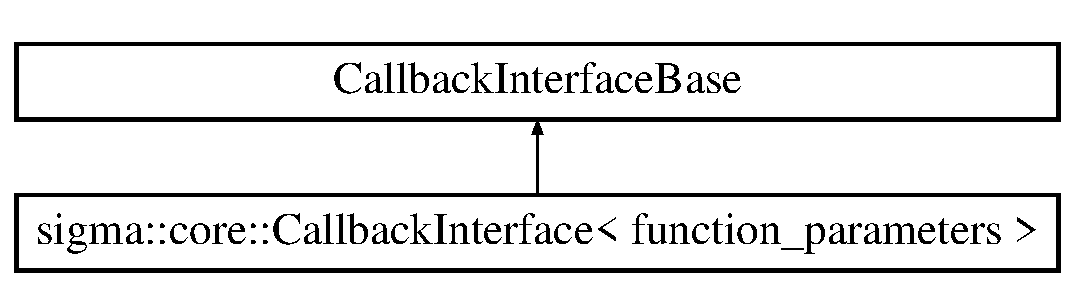
\includegraphics[height=2.000000cm]{classsigma_1_1core_1_1_callback_interface}
\end{center}
\end{figure}
\subsection*{Public Member Functions}
\begin{DoxyCompactItemize}
\item 
\hyperlink{classsigma_1_1core_1_1_scoped_callback}{Scoped\+Callback} \hyperlink{classsigma_1_1core_1_1_callback_interface_a1117c0ac1a539abfe254e2f12dc1880d}{register\+\_\+function} (void($\ast$callback\+\_\+function)(function\+\_\+parameters...))
\begin{DoxyCompactList}\small\item\em Registers a global or static function as a callback. \end{DoxyCompactList}\item 
{\footnotesize template$<$typename owner\+\_\+type , void(owner\+\_\+type\+::$\ast$)(function\+\_\+parameters...) function\+\_\+type$>$ }\\\hyperlink{classsigma_1_1core_1_1_scoped_callback}{Scoped\+Callback} \hyperlink{classsigma_1_1core_1_1_callback_interface_aaa44a699001122a4828013af440345c7}{register\+\_\+member\+\_\+function} (owner\+\_\+type $\ast$owner)
\begin{DoxyCompactList}\small\item\em Registers a member function as a callback. \end{DoxyCompactList}\end{DoxyCompactItemize}
\subsection*{Friends}
\begin{DoxyCompactItemize}
\item 
\hypertarget{classsigma_1_1core_1_1_callback_interface_a3414685dbc2eaa79d5e5af6729f74c0f}{}class {\bfseries Scoped\+Callback}\label{classsigma_1_1core_1_1_callback_interface_a3414685dbc2eaa79d5e5af6729f74c0f}

\item 
\hypertarget{classsigma_1_1core_1_1_callback_interface_aa40ef6fe1ae370543551561772e9d468}{}class {\bfseries Callback\+Handler$<$ function\+\_\+parameters... $>$}\label{classsigma_1_1core_1_1_callback_interface_aa40ef6fe1ae370543551561772e9d468}

\end{DoxyCompactItemize}


\subsection{Detailed Description}
\subsubsection*{template$<$typename... function\+\_\+parameters$>$class sigma\+::core\+::\+Callback\+Interface$<$ function\+\_\+parameters $>$}

Used to register global, static, and member functions as callbacks. 

This object will call all registered callback functions when triggered. The callback routine may only be triggered by the owner of this object, see\+: \hyperlink{classsigma_1_1core_1_1_callback_handler}{sigma\+::core\+::\+Callback\+Handler}.

Registered functions are manager through \hyperlink{classsigma_1_1core_1_1_scoped_callback}{sigma\+::core\+::\+Scoped\+Callback} instances which aid managing the lifetime of the callback.

An example of registering both a global and a member function callback\+:


\begin{DoxyCode}
\textcolor{comment}{// g\_callback\_interface is an object of type CallbackInterface<bool, int>}

\textcolor{keywordtype}{void} global\_callback\_func(\textcolor{keywordtype}{bool} a, \textcolor{keywordtype}{int} b)
\{
    std::cout << \textcolor{stringliteral}{"global called: "} << a << \textcolor{stringliteral}{":"} << b << std::endl;
\}

\textcolor{keyword}{class }MyClass
\{
\textcolor{keyword}{public}:

    \textcolor{keywordtype}{void} member\_callback\_function(\textcolor{keywordtype}{bool} a, \textcolor{keywordtype}{int} b)
    \{
        std::cout << \textcolor{stringliteral}{"member called: "} << a << \textcolor{stringliteral}{":"} << b << std::endl;
    \}
\}

\textcolor{keywordtype}{int} main(\textcolor{keywordtype}{int} argc, \textcolor{keywordtype}{char}* argv[])
\{
    MyClass my\_class;

    \hyperlink{classsigma_1_1core_1_1_scoped_callback}{sigma::core::ScopedCallback} callback\_1(
            g\_callback\_interface.register\_function(global\_callback\_func)
    );
    \hyperlink{classsigma_1_1core_1_1_scoped_callback}{sigma::core::ScopedCallback} callback\_1(
            g\_callback\_interface.register\_member\_function<
                    <MyClass, &MyClass::member\_callback\_function>(&my\_class)
    );

    \textcolor{keywordflow}{return} 0;
\}
\end{DoxyCode}


Notice that the global function may be passed in directly to the {\ttfamily register\+\_\+function method}, but the member function must be passed in using templates. This is because member function pointers are treated differently to function pointers in C++. The {\ttfamily register\+\_\+member\+\_\+function} needs to know the member functions class type (template parameter 1), the member function to call (template parameter 2), and the object instance to call the member function on (function parameter 1).


\begin{DoxyTemplParams}{Template Parameters}
{\em function\+\_\+parameters} & The types of the parameters of the function this \hyperlink{classsigma_1_1core_1_1_callback_interface}{Callback\+Interface} is managing. \\
\hline
\end{DoxyTemplParams}


\subsection{Member Function Documentation}
\hypertarget{classsigma_1_1core_1_1_callback_interface_a1117c0ac1a539abfe254e2f12dc1880d}{}\index{sigma\+::core\+::\+Callback\+Interface@{sigma\+::core\+::\+Callback\+Interface}!register\+\_\+function@{register\+\_\+function}}
\index{register\+\_\+function@{register\+\_\+function}!sigma\+::core\+::\+Callback\+Interface@{sigma\+::core\+::\+Callback\+Interface}}
\subsubsection[{register\+\_\+function(void($\ast$callback\+\_\+function)(function\+\_\+parameters...))}]{\setlength{\rightskip}{0pt plus 5cm}template$<$typename... function\+\_\+parameters$>$ {\bf Scoped\+Callback} {\bf sigma\+::core\+::\+Callback\+Interface}$<$ function\+\_\+parameters $>$\+::register\+\_\+function (
\begin{DoxyParamCaption}
\item[{void($\ast$)(function\+\_\+parameters...)}]{callback\+\_\+function}
\end{DoxyParamCaption}
)\hspace{0.3cm}{\ttfamily [inline]}}\label{classsigma_1_1core_1_1_callback_interface_a1117c0ac1a539abfe254e2f12dc1880d}


Registers a global or static function as a callback. 

Registered functions will be called when callback owner triggers the \hyperlink{classsigma_1_1core_1_1_callback_handler}{Callback\+Handler}.


\begin{DoxyParams}{Parameters}
{\em callback\+\_\+function} & The function to register as callback.\\
\hline
\end{DoxyParams}
\begin{DoxyReturn}{Returns}
A \hyperlink{classsigma_1_1core_1_1_scoped_callback}{sigma\+::core\+::\+Scoped\+Callback} which is used to unregister this callback. 
\end{DoxyReturn}
\hypertarget{classsigma_1_1core_1_1_callback_interface_aaa44a699001122a4828013af440345c7}{}\index{sigma\+::core\+::\+Callback\+Interface@{sigma\+::core\+::\+Callback\+Interface}!register\+\_\+member\+\_\+function@{register\+\_\+member\+\_\+function}}
\index{register\+\_\+member\+\_\+function@{register\+\_\+member\+\_\+function}!sigma\+::core\+::\+Callback\+Interface@{sigma\+::core\+::\+Callback\+Interface}}
\subsubsection[{register\+\_\+member\+\_\+function(owner\+\_\+type $\ast$owner)}]{\setlength{\rightskip}{0pt plus 5cm}template$<$typename... function\+\_\+parameters$>$ template$<$typename owner\+\_\+type , void(owner\+\_\+type\+::$\ast$)(function\+\_\+parameters...) function\+\_\+type$>$ {\bf Scoped\+Callback} {\bf sigma\+::core\+::\+Callback\+Interface}$<$ function\+\_\+parameters $>$\+::register\+\_\+member\+\_\+function (
\begin{DoxyParamCaption}
\item[{owner\+\_\+type $\ast$}]{owner}
\end{DoxyParamCaption}
)\hspace{0.3cm}{\ttfamily [inline]}}\label{classsigma_1_1core_1_1_callback_interface_aaa44a699001122a4828013af440345c7}


Registers a member function as a callback. 

Registered functions will be called when callback owner triggers the \hyperlink{classsigma_1_1core_1_1_callback_handler}{Callback\+Handler}.

See \hyperlink{classsigma_1_1core_1_1_callback_interface}{sigma\+::core\+::\+Callback\+Interface} for a usage example.


\begin{DoxyTemplParams}{Template Parameters}
{\em owner\+\_\+type} & The class type that the member function is part of. \\
\hline
{\em function\+\_\+type} & The member function type to register as a callback. \\
\hline
\end{DoxyTemplParams}

\begin{DoxyParams}{Parameters}
{\em owner} & Instance of the object that owns the member function to be used as the callback.\\
\hline
\end{DoxyParams}
\begin{DoxyReturn}{Returns}
A \hyperlink{classsigma_1_1core_1_1_scoped_callback}{sigma\+::core\+::\+Scoped\+Callback} which is used to unregister this callback. 
\end{DoxyReturn}


The documentation for this class was generated from the following file\+:\begin{DoxyCompactItemize}
\item 
D\+:/\+Dropbox/\+Development/\+Sigma/\+Sigma/src/cxx/sigma/core/\hyperlink{_callback_8hpp}{Callback.\+hpp}\end{DoxyCompactItemize}

\hypertarget{classsigma_1_1core_1_1tasks_1_1_root_task}{}\section{sigma\+:\+:core\+:\+:tasks\+:\+:Root\+Task Class Reference}
\label{classsigma_1_1core_1_1tasks_1_1_root_task}\index{sigma\+::core\+::tasks\+::\+Root\+Task@{sigma\+::core\+::tasks\+::\+Root\+Task}}


T\+O\+D\+O.  




{\ttfamily \#include $<$Root\+Task.\+hpp$>$}

Inheritance diagram for sigma\+:\+:core\+:\+:tasks\+:\+:Root\+Task\+:\begin{figure}[H]
\begin{center}
\leavevmode
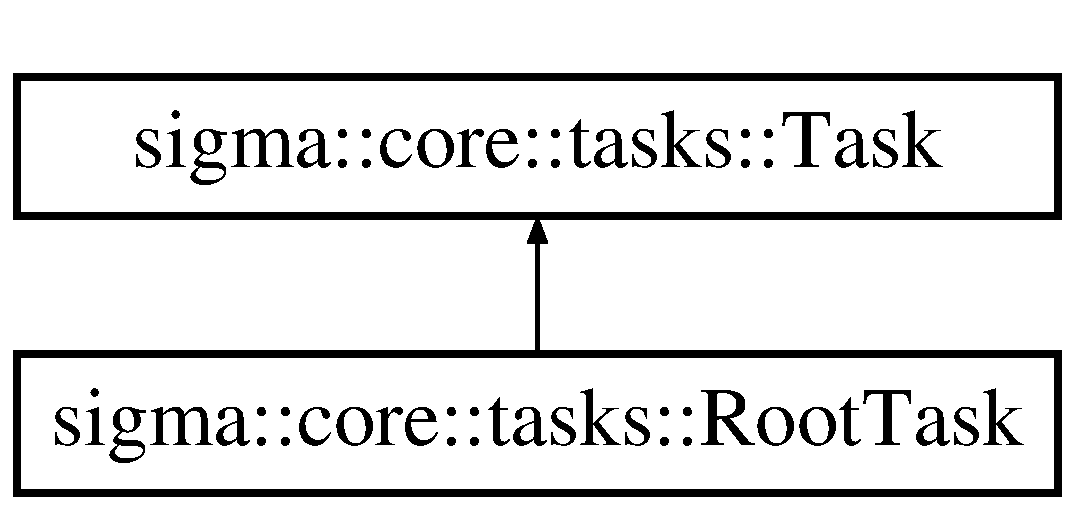
\includegraphics[height=2.000000cm]{classsigma_1_1core_1_1tasks_1_1_root_task}
\end{center}
\end{figure}
\subsection*{Public Member Functions}
\begin{DoxyCompactItemize}
\item 
\hypertarget{classsigma_1_1core_1_1tasks_1_1_root_task_a121303d6c4380323fe54bc823ef11514}{}virtual bool \hyperlink{classsigma_1_1core_1_1tasks_1_1_root_task_a121303d6c4380323fe54bc823ef11514}{is\+\_\+root} () const \label{classsigma_1_1core_1_1tasks_1_1_root_task_a121303d6c4380323fe54bc823ef11514}

\begin{DoxyCompactList}\small\item\em Returns whether this is a \hyperlink{classsigma_1_1core_1_1tasks_1_1_root_task}{Root\+Task} or not. \end{DoxyCompactList}\item 
\hypertarget{classsigma_1_1core_1_1tasks_1_1_root_task_a4b9f9c86ba7a0e5b681479a444cd60b1}{}virtual void \hyperlink{classsigma_1_1core_1_1tasks_1_1_root_task_a4b9f9c86ba7a0e5b681479a444cd60b1}{set\+\_\+parent} (\hyperlink{classsigma_1_1core_1_1tasks_1_1_task}{Task} $\ast$const parent)\label{classsigma_1_1core_1_1tasks_1_1_root_task_a4b9f9c86ba7a0e5b681479a444cd60b1}

\begin{DoxyCompactList}\small\item\em Throws an arc\+::ex\+::\+Illegal\+Action\+Error since a \hyperlink{classsigma_1_1core_1_1tasks_1_1_root_task}{Root\+Task} cannot have a parent. \end{DoxyCompactList}\item 
\hypertarget{classsigma_1_1core_1_1tasks_1_1_root_task_a825247badddb1934e51ace7df99503f3}{}virtual void \hyperlink{classsigma_1_1core_1_1tasks_1_1_root_task_a825247badddb1934e51ace7df99503f3}{set\+\_\+title} (const arc\+::str\+::\+U\+T\+F8\+String \&title)\label{classsigma_1_1core_1_1tasks_1_1_root_task_a825247badddb1934e51ace7df99503f3}

\begin{DoxyCompactList}\small\item\em Sets the title string of this \hyperlink{classsigma_1_1core_1_1tasks_1_1_task}{Task}. \end{DoxyCompactList}\end{DoxyCompactItemize}
\subsection*{Friends}
\begin{DoxyCompactItemize}
\item 
\hypertarget{classsigma_1_1core_1_1tasks_1_1_root_task_aa9cd0697dba448e5a3349d45503a9239}{}\hyperlink{classsigma_1_1core_1_1tasks_1_1_root_task}{Root\+Task} $\ast$ {\bfseries domain\+::new\+\_\+board} (const arc\+::str\+::\+U\+T\+F8\+String \&)\label{classsigma_1_1core_1_1tasks_1_1_root_task_aa9cd0697dba448e5a3349d45503a9239}

\end{DoxyCompactItemize}
\subsection*{Additional Inherited Members}


\subsection{Detailed Description}
T\+O\+D\+O. 

T\+O\+D\+O\+: 

The documentation for this class was generated from the following file\+:\begin{DoxyCompactItemize}
\item 
D\+:/\+Dropbox/\+Development/\+Sigma/\+Sigma/src/cpp/sigma/core/tasks/\hyperlink{_root_task_8hpp}{Root\+Task.\+hpp}\end{DoxyCompactItemize}

\hypertarget{classsigma_1_1core_1_1_scoped_callback}{}\section{sigma\+:\+:core\+:\+:Scoped\+Callback Class Reference}
\label{classsigma_1_1core_1_1_scoped_callback}\index{sigma\+::core\+::\+Scoped\+Callback@{sigma\+::core\+::\+Scoped\+Callback}}


Object that holds the id of a callback function and aids in life cycle management of the callback.  




{\ttfamily \#include $<$Callback.\+hpp$>$}

\subsection*{Public Member Functions}
\begin{DoxyCompactItemize}
\item 
\hyperlink{classsigma_1_1core_1_1_scoped_callback_ae39d91862f76b1804acc8edae410678e}{Scoped\+Callback} (const \hyperlink{classsigma_1_1core_1_1_scoped_callback}{Scoped\+Callback} \&other)
\begin{DoxyCompactList}\small\item\em Copy constructor. \end{DoxyCompactList}\item 
\hypertarget{classsigma_1_1core_1_1_scoped_callback_ab0eabc2e0c158643758501f9c6bc444c}{}\hyperlink{classsigma_1_1core_1_1_scoped_callback}{Scoped\+Callback} \& {\bfseries operator=} (const \hyperlink{classsigma_1_1core_1_1_scoped_callback}{Scoped\+Callback} \&other)=delete\label{classsigma_1_1core_1_1_scoped_callback_ab0eabc2e0c158643758501f9c6bc444c}

\item 
\hypertarget{classsigma_1_1core_1_1_scoped_callback_a3b4ae371184bb639999677cf66440461}{}chaos\+::uint32 \hyperlink{classsigma_1_1core_1_1_scoped_callback_a3b4ae371184bb639999677cf66440461}{get\+\_\+id} () const \label{classsigma_1_1core_1_1_scoped_callback_a3b4ae371184bb639999677cf66440461}

\begin{DoxyCompactList}\small\item\em Returns the id of this callback. \end{DoxyCompactList}\item 
bool \hyperlink{classsigma_1_1core_1_1_scoped_callback_adafe2e52e653bca84d11f1d0baaec616}{is\+\_\+registered} () const 
\begin{DoxyCompactList}\small\item\em Returns whether this contains a registered callback or not. \end{DoxyCompactList}\item 
void \hyperlink{classsigma_1_1core_1_1_scoped_callback_ad8d8ea4671f58077c8f9ef020e52e125}{unregister} ()
\begin{DoxyCompactList}\small\item\em Explicitly unregisters this callback. \end{DoxyCompactList}\end{DoxyCompactItemize}


\subsection{Detailed Description}
Object that holds the id of a callback function and aids in life cycle management of the callback. 

\hyperlink{classsigma_1_1core_1_1_scoped_callback}{Scoped\+Callback}\textquotesingle{}s use reference counting to manage the life cycle of the callback. Once all references to this callback go out of scope or are destroyed the Callback will be unregistered.

The \hyperlink{classsigma_1_1core_1_1_scoped_callback}{Scoped\+Callback} can be explicitly unregistered using the {\ttfamily unregister} function. Once explicitly unregistered other reference to this are safe to go out of scope and have the {\ttfamily unregister} function called on them (although redundant). 

\subsection{Constructor \& Destructor Documentation}
\hypertarget{classsigma_1_1core_1_1_scoped_callback_ae39d91862f76b1804acc8edae410678e}{}\index{sigma\+::core\+::\+Scoped\+Callback@{sigma\+::core\+::\+Scoped\+Callback}!Scoped\+Callback@{Scoped\+Callback}}
\index{Scoped\+Callback@{Scoped\+Callback}!sigma\+::core\+::\+Scoped\+Callback@{sigma\+::core\+::\+Scoped\+Callback}}
\subsubsection[{Scoped\+Callback(const Scoped\+Callback \&other)}]{\setlength{\rightskip}{0pt plus 5cm}sigma\+::core\+::\+Scoped\+Callback\+::\+Scoped\+Callback (
\begin{DoxyParamCaption}
\item[{const {\bf Scoped\+Callback} \&}]{other}
\end{DoxyParamCaption}
)\hspace{0.3cm}{\ttfamily [inline]}}\label{classsigma_1_1core_1_1_scoped_callback_ae39d91862f76b1804acc8edae410678e}


Copy constructor. 

Makes a copy of the given \hyperlink{classsigma_1_1core_1_1_scoped_callback}{Scoped\+Callback} and increases the reference counter. 

\subsection{Member Function Documentation}
\hypertarget{classsigma_1_1core_1_1_scoped_callback_adafe2e52e653bca84d11f1d0baaec616}{}\index{sigma\+::core\+::\+Scoped\+Callback@{sigma\+::core\+::\+Scoped\+Callback}!is\+\_\+registered@{is\+\_\+registered}}
\index{is\+\_\+registered@{is\+\_\+registered}!sigma\+::core\+::\+Scoped\+Callback@{sigma\+::core\+::\+Scoped\+Callback}}
\subsubsection[{is\+\_\+registered() const }]{\setlength{\rightskip}{0pt plus 5cm}bool sigma\+::core\+::\+Scoped\+Callback\+::is\+\_\+registered (
\begin{DoxyParamCaption}
{}
\end{DoxyParamCaption}
) const\hspace{0.3cm}{\ttfamily [inline]}}\label{classsigma_1_1core_1_1_scoped_callback_adafe2e52e653bca84d11f1d0baaec616}


Returns whether this contains a registered callback or not. 

A callback may return as unregistered because\+:
\begin{DoxyItemize}
\item {\ttfamily unregister} has been explicitly called.
\item The {\ttfamily \hyperlink{classsigma_1_1core_1_1_callback_handler}{Callback\+Handler}}/{\ttfamily \hyperlink{classsigma_1_1core_1_1_callback_interface}{Callback\+Interface}} this was registered with has been destroyed. 
\end{DoxyItemize}\hypertarget{classsigma_1_1core_1_1_scoped_callback_ad8d8ea4671f58077c8f9ef020e52e125}{}\index{sigma\+::core\+::\+Scoped\+Callback@{sigma\+::core\+::\+Scoped\+Callback}!unregister@{unregister}}
\index{unregister@{unregister}!sigma\+::core\+::\+Scoped\+Callback@{sigma\+::core\+::\+Scoped\+Callback}}
\subsubsection[{unregister()}]{\setlength{\rightskip}{0pt plus 5cm}void sigma\+::core\+::\+Scoped\+Callback\+::unregister (
\begin{DoxyParamCaption}
{}
\end{DoxyParamCaption}
)\hspace{0.3cm}{\ttfamily [inline]}}\label{classsigma_1_1core_1_1_scoped_callback_ad8d8ea4671f58077c8f9ef020e52e125}


Explicitly unregisters this callback. 

Once the callback has been unregistered the function this is associated with will no longer be called when the \hyperlink{classsigma_1_1core_1_1_callback_handler}{Callback\+Handler} is triggered.

This function is safe to call multiple times although additional calls are redundant and have no further affect. 

The documentation for this class was generated from the following file\+:\begin{DoxyCompactItemize}
\item 
D\+:/\+Dropbox/\+Development/\+Sigma/\+Sigma/src/cxx/sigma/core/\hyperlink{_callback_8hpp}{Callback.\+hpp}\end{DoxyCompactItemize}

\hypertarget{classsigma_1_1gui_1_1startup_1_1_splash_screen}{\section{sigma\-:\-:gui\-:\-:startup\-:\-:Splash\-Screen Class Reference}
\label{classsigma_1_1gui_1_1startup_1_1_splash_screen}\index{sigma\-::gui\-::startup\-::\-Splash\-Screen@{sigma\-::gui\-::startup\-::\-Splash\-Screen}}
}


Base widget for the Sigma startup splash screen.  




{\ttfamily \#include $<$Splash\-Screen.\-hpp$>$}

Inheritance diagram for sigma\-:\-:gui\-:\-:startup\-:\-:Splash\-Screen\-:\begin{figure}[H]
\begin{center}
\leavevmode
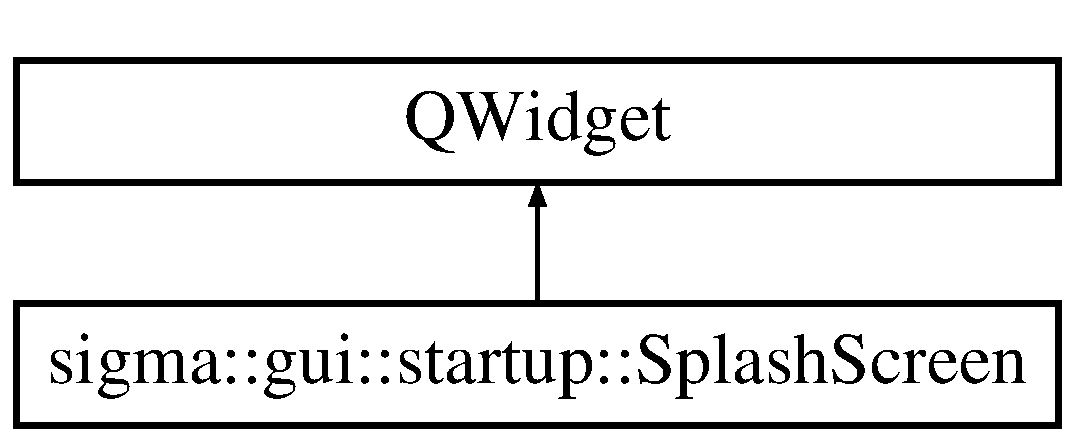
\includegraphics[height=2.000000cm]{classsigma_1_1gui_1_1startup_1_1_splash_screen}
\end{center}
\end{figure}


\subsection{Detailed Description}
Base widget for the Sigma startup splash screen. 

The documentation for this class was generated from the following file\-:\begin{DoxyCompactItemize}
\item 
/home/david/\-Dropbox/\-Development/\-Sigma/\-Sigma/src/cpp/sigma/gui/startup/\hyperlink{_splash_screen_8hpp}{Splash\-Screen.\-hpp}\end{DoxyCompactItemize}

\hypertarget{classsigma_1_1core_1_1tasks_1_1_task}{}\section{sigma\+:\+:core\+:\+:tasks\+:\+:Task Class Reference}
\label{classsigma_1_1core_1_1tasks_1_1_task}\index{sigma\+::core\+::tasks\+::\+Task@{sigma\+::core\+::tasks\+::\+Task}}


T\+O\+D\+O.  




{\ttfamily \#include $<$Task.\+hpp$>$}

\subsection*{Public Member Functions}
\begin{DoxyCompactItemize}
\item 
\hyperlink{classsigma_1_1core_1_1tasks_1_1_task_a0e0bb9899317a89bf9e49bd04513bc04}{Task} (const chaos\+::uni\+::\+U\+T\+F8\+String \&title, \hyperlink{classsigma_1_1core_1_1tasks_1_1_task}{Task} $\ast$parent=nullptr)
\begin{DoxyCompactList}\small\item\em T\+O\+D\+O. \end{DoxyCompactList}\item 
\hypertarget{classsigma_1_1core_1_1tasks_1_1_task_a8fd41c73909654ee57670b45c273a65b}{}const chaos\+::uni\+::\+U\+T\+F8\+String \& {\bfseries get\+\_\+title} () const \label{classsigma_1_1core_1_1tasks_1_1_task_a8fd41c73909654ee57670b45c273a65b}

\item 
\hypertarget{classsigma_1_1core_1_1tasks_1_1_task_a1f17b3e1f7b444d6a73f5391e929adc5}{}void {\bfseries set\+\_\+title} (const chaos\+::uni\+::\+U\+T\+F8\+String \&title)\label{classsigma_1_1core_1_1tasks_1_1_task_a1f17b3e1f7b444d6a73f5391e929adc5}

\item 
\hypertarget{classsigma_1_1core_1_1tasks_1_1_task_ae954c977b0085755d73ef44073152fec}{}\hyperlink{classsigma_1_1core_1_1_callback_interface}{sigma\+::core\+::\+Callback\+Interface}$<$ \hyperlink{classsigma_1_1core_1_1tasks_1_1_task}{Task} $\ast$, const chaos\+::uni\+::\+U\+T\+F8\+String \& $>$ $\ast$ \hyperlink{classsigma_1_1core_1_1tasks_1_1_task_ae954c977b0085755d73ef44073152fec}{on\+\_\+title\+\_\+changed} ()\label{classsigma_1_1core_1_1tasks_1_1_task_ae954c977b0085755d73ef44073152fec}

\begin{DoxyCompactList}\small\item\em T\+O\+D\+O. \end{DoxyCompactList}\end{DoxyCompactItemize}
\subsection*{Static Public Member Functions}
\begin{DoxyCompactItemize}
\item 
\hypertarget{classsigma_1_1core_1_1tasks_1_1_task_ab5adda36bbe6b20916f582ffeb311a13}{}static \hyperlink{classsigma_1_1core_1_1_callback_interface}{sigma\+::core\+::\+Callback\+Interface}$<$ \hyperlink{classsigma_1_1core_1_1tasks_1_1_task}{Task} $\ast$ $>$ $\ast$ \hyperlink{classsigma_1_1core_1_1tasks_1_1_task_ab5adda36bbe6b20916f582ffeb311a13}{on\+\_\+created} ()\label{classsigma_1_1core_1_1tasks_1_1_task_ab5adda36bbe6b20916f582ffeb311a13}

\begin{DoxyCompactList}\small\item\em T\+O\+D\+O. \end{DoxyCompactList}\item 
\hypertarget{classsigma_1_1core_1_1tasks_1_1_task_a720571d12a0e2b41c918f448f5fc81db}{}static \hyperlink{classsigma_1_1core_1_1_callback_interface}{sigma\+::core\+::\+Callback\+Interface}$<$ \hyperlink{classsigma_1_1core_1_1tasks_1_1_task}{Task} $\ast$ $>$ $\ast$ \hyperlink{classsigma_1_1core_1_1tasks_1_1_task_a720571d12a0e2b41c918f448f5fc81db}{on\+\_\+destroyed} ()\label{classsigma_1_1core_1_1tasks_1_1_task_a720571d12a0e2b41c918f448f5fc81db}

\begin{DoxyCompactList}\small\item\em T\+O\+D\+O. \end{DoxyCompactList}\end{DoxyCompactItemize}


\subsection{Detailed Description}
T\+O\+D\+O. 

T\+O\+D\+O 

\subsection{Constructor \& Destructor Documentation}
\hypertarget{classsigma_1_1core_1_1tasks_1_1_task_a0e0bb9899317a89bf9e49bd04513bc04}{}\index{sigma\+::core\+::tasks\+::\+Task@{sigma\+::core\+::tasks\+::\+Task}!Task@{Task}}
\index{Task@{Task}!sigma\+::core\+::tasks\+::\+Task@{sigma\+::core\+::tasks\+::\+Task}}
\subsubsection[{Task(const chaos\+::uni\+::\+U\+T\+F8\+String \&title, Task $\ast$parent=nullptr)}]{\setlength{\rightskip}{0pt plus 5cm}sigma\+::core\+::tasks\+::\+Task\+::\+Task (
\begin{DoxyParamCaption}
\item[{const chaos\+::uni\+::\+U\+T\+F8\+String \&}]{title, }
\item[{{\bf Task} $\ast$}]{parent = {\ttfamily nullptr}}
\end{DoxyParamCaption}
)}\label{classsigma_1_1core_1_1tasks_1_1_task_a0e0bb9899317a89bf9e49bd04513bc04}


T\+O\+D\+O. 

T\+O\+D\+O 

The documentation for this class was generated from the following file\+:\begin{DoxyCompactItemize}
\item 
D\+:/\+Dropbox/\+Development/\+Sigma/\+Sigma/src/cxx/sigma/core/tasks/\hyperlink{_task_8hpp}{Task.\+hpp}\end{DoxyCompactItemize}

\chapter{File Documentation}
\hypertarget{_callback_8hpp}{\section{/home/david/\-Dropbox/\-Development/\-Sigma/\-Sigma/src/cxx/sigma/core/\-Callback.hpp File Reference}
\label{_callback_8hpp}\index{/home/david/\-Dropbox/\-Development/\-Sigma/\-Sigma/src/cxx/sigma/core/\-Callback.\-hpp@{/home/david/\-Dropbox/\-Development/\-Sigma/\-Sigma/src/cxx/sigma/core/\-Callback.\-hpp}}
}
{\ttfamily \#include $<$cassert$>$}\\*
{\ttfamily \#include $<$map$>$}\\*
{\ttfamily \#include $<$memory$>$}\\*
{\ttfamily \#include $<$chaoscore/base/\-Base\-Exceptions.\-hpp$>$}\\*
{\ttfamily \#include $<$iostream$>$}\\*
\subsection*{Classes}
\begin{DoxyCompactItemize}
\item 
class \hyperlink{classsigma_1_1core_1_1_callback_handler}{sigma\-::core\-::\-Callback\-Handler$<$ function\-\_\-parameters $>$}
\begin{DoxyCompactList}\small\item\em Object used to handle callbacks of a given function type. \end{DoxyCompactList}\item 
class \hyperlink{classsigma_1_1core_1_1_scoped_callback}{sigma\-::core\-::\-Scoped\-Callback}
\begin{DoxyCompactList}\small\item\em Object that holds the id of a callback function and aids in life cycle management of the callback. \end{DoxyCompactList}\item 
class \hyperlink{classsigma_1_1core_1_1_callback_interface}{sigma\-::core\-::\-Callback\-Interface$<$ function\-\_\-parameters $>$}
\begin{DoxyCompactList}\small\item\em Used to register global, static, and member functions as callbacks. \end{DoxyCompactList}\item 
class \hyperlink{classsigma_1_1core_1_1_callback_handler}{sigma\-::core\-::\-Callback\-Handler$<$ function\-\_\-parameters $>$}
\begin{DoxyCompactList}\small\item\em Object used to handle callbacks of a given function type. \end{DoxyCompactList}\end{DoxyCompactItemize}
\subsection*{Namespaces}
\begin{DoxyCompactItemize}
\item 
\hyperlink{namespacesigma}{sigma}
\begin{DoxyCompactList}\small\item\em the global namespace which contains all built-\/in aspects of Sigma. \end{DoxyCompactList}\item 
\hyperlink{namespacesigma_1_1core}{sigma\-::core}
\begin{DoxyCompactList}\small\item\em The core backend A\-P\-I of Sigma. Sigma core is entirely detached from any Sigma U\-I. \end{DoxyCompactList}\end{DoxyCompactItemize}


\subsection{Detailed Description}
\begin{DoxyAuthor}{Author}
David Saxon 
\end{DoxyAuthor}

\hypertarget{_core_logging_8hpp}{}\section{D\+:/\+Dropbox/\+Development/\+Sigma/\+Sigma/src/cpp/sigma/core/\+Core\+Logging.hpp File Reference}
\label{_core_logging_8hpp}\index{D\+:/\+Dropbox/\+Development/\+Sigma/\+Sigma/src/cpp/sigma/core/\+Core\+Logging.\+hpp@{D\+:/\+Dropbox/\+Development/\+Sigma/\+Sigma/src/cpp/sigma/core/\+Core\+Logging.\+hpp}}


Logging in relation to Sigma\textquotesingle{}s core.  




\subsection{Detailed Description}
Logging in relation to Sigma\textquotesingle{}s core. 

\begin{DoxyAuthor}{Author}
David Saxon 
\end{DoxyAuthor}

\hypertarget{_sigma_8hpp}{\section{/home/david/\-Dropbox/\-Development/\-Sigma/\-Sigma/src/cxx/sigma/core/\-Sigma.hpp File Reference}
\label{_sigma_8hpp}\index{/home/david/\-Dropbox/\-Development/\-Sigma/\-Sigma/src/cxx/sigma/core/\-Sigma.\-hpp@{/home/david/\-Dropbox/\-Development/\-Sigma/\-Sigma/src/cxx/sigma/core/\-Sigma.\-hpp}}
}


The main entry point for the Sigma A\-P\-I.  


\subsection*{Namespaces}
\begin{DoxyCompactItemize}
\item 
\hyperlink{namespacesigma}{sigma}
\begin{DoxyCompactList}\small\item\em the global namespace which contains all built-\/in aspects of Sigma. \end{DoxyCompactList}\item 
\hyperlink{namespacesigma_1_1core}{sigma\-::core}
\begin{DoxyCompactList}\small\item\em The core backend A\-P\-I of Sigma. Sigma core is entirely detached from any Sigma U\-I. \end{DoxyCompactList}\end{DoxyCompactItemize}
\subsection*{Enumerations}
\begin{DoxyCompactItemize}
\item 
enum \hyperlink{namespacesigma_1_1core_a48ec553a4adec5e4ca04a94946e39227}{sigma\-::core\-::\-A\-P\-I\-Domains} \{ \\*
\hyperlink{namespacesigma_1_1core_a48ec553a4adec5e4ca04a94946e39227ad5c128a2a2f3f1354dc44fd6e477b2c9}{sigma\-::core\-::\-A\-P\-I\-\_\-\-N\-O\-N\-E}, 
\hyperlink{namespacesigma_1_1core_a48ec553a4adec5e4ca04a94946e39227a21b294c75f929374e9eebfa67e31d80b}{sigma\-::core\-::\-A\-P\-I\-\_\-\-B\-U\-I\-L\-D}, 
\hyperlink{namespacesigma_1_1core_a48ec553a4adec5e4ca04a94946e39227acd512ee6c623f9c4b6faafc279cb93c8}{sigma\-::core\-::\-A\-P\-I\-\_\-\-T\-E\-S\-T}, 
\hyperlink{namespacesigma_1_1core_a48ec553a4adec5e4ca04a94946e39227a165d0d460d4f55091c38bab695b27bb4}{sigma\-::core\-::\-A\-P\-I\-\_\-\-T\-A\-S\-K\-S}, 
\\*
\hyperlink{namespacesigma_1_1core_a48ec553a4adec5e4ca04a94946e39227aac7402732b780aa9407183ed7bd7c809}{sigma\-::core\-::\-A\-P\-I\-\_\-\-L\-I\-N\-T}, 
\hyperlink{namespacesigma_1_1core_a48ec553a4adec5e4ca04a94946e39227a5328f8d7cbf6b6709e5f314832bcb007}{sigma\-::core\-::\-A\-P\-I\-\_\-\-A\-L\-L}
 \}
\begin{DoxyCompactList}\small\item\em The built-\/in A\-P\-I domains of Sigma. \end{DoxyCompactList}\end{DoxyCompactItemize}
\subsection*{Functions}
\begin{DoxyCompactItemize}
\item 
void \hyperlink{namespacesigma_1_1core_ae59ffd8d8b483f24878a0bf7425c436c}{sigma\-::core\-::init} (A\-P\-I\-Domains api\-\_\-domains=A\-P\-I\-\_\-\-A\-L\-L)
\begin{DoxyCompactList}\small\item\em Initialises Sigma. \end{DoxyCompactList}\end{DoxyCompactItemize}


\subsection{Detailed Description}
The main entry point for the Sigma A\-P\-I. \begin{DoxyAuthor}{Author}
David Saxon Most importantly this file provides the init function which must be called before Sigma can be used. 
\end{DoxyAuthor}

\hypertarget{_root_task_8hpp}{\section{/home/david/\-Dropbox/\-Development/\-Sigma/\-Sigma/src/cpp/sigma/core/tasks/\-Root\-Task.hpp File Reference}
\label{_root_task_8hpp}\index{/home/david/\-Dropbox/\-Development/\-Sigma/\-Sigma/src/cpp/sigma/core/tasks/\-Root\-Task.\-hpp@{/home/david/\-Dropbox/\-Development/\-Sigma/\-Sigma/src/cpp/sigma/core/tasks/\-Root\-Task.\-hpp}}
}
{\ttfamily \#include \char`\"{}sigma/core/tasks/\-Task.\-hpp\char`\"{}}\\*
{\ttfamily \#include \char`\"{}sigma/core/tasks/\-Tasks\-Domain.\-hpp\char`\"{}}\\*
\subsection*{Classes}
\begin{DoxyCompactItemize}
\item 
class \hyperlink{classsigma_1_1core_1_1tasks_1_1_root_task}{sigma\-::core\-::tasks\-::\-Root\-Task}
\begin{DoxyCompactList}\small\item\em T\-O\-D\-O. \end{DoxyCompactList}\end{DoxyCompactItemize}
\subsection*{Namespaces}
\begin{DoxyCompactItemize}
\item 
\hyperlink{namespacesigma}{sigma}
\begin{DoxyCompactList}\small\item\em the global namespace which contains all built-\/in aspects of Sigma. \end{DoxyCompactList}\item 
\hyperlink{namespacesigma_1_1core}{sigma\-::core}
\begin{DoxyCompactList}\small\item\em The core backend A\-P\-I of Sigma. Sigma core is entirely detached from any Sigma U\-I. \end{DoxyCompactList}\item 
\hyperlink{namespacesigma_1_1core_1_1tasks}{sigma\-::core\-::tasks}
\begin{DoxyCompactList}\small\item\em The task management A\-P\-I module of Sigma. \end{DoxyCompactList}\end{DoxyCompactItemize}
\subsection*{Typedefs}
\begin{DoxyCompactItemize}
\item 
\hypertarget{namespacesigma_1_1core_1_1tasks_a39960f0c083a360cafd859f4f394ff8e}{typedef void($\ast$ {\bfseries sigma\-::core\-::tasks\-::\-Title\-Resolver\-\_\-t} )(const arc\-::str\-::\-U\-T\-F8\-String \&, arc\-::str\-::\-U\-T\-F8\-String \&)}\label{namespacesigma_1_1core_1_1tasks_a39960f0c083a360cafd859f4f394ff8e}

\end{DoxyCompactItemize}


\subsection{Detailed Description}
\begin{DoxyAuthor}{Author}
David Saxon 
\end{DoxyAuthor}

\hypertarget{_task_8hpp}{}\section{D\+:/\+Dropbox/\+Development/\+Sigma/\+Sigma/src/cxx/sigma/core/tasks/\+Task.hpp File Reference}
\label{_task_8hpp}\index{D\+:/\+Dropbox/\+Development/\+Sigma/\+Sigma/src/cxx/sigma/core/tasks/\+Task.\+hpp@{D\+:/\+Dropbox/\+Development/\+Sigma/\+Sigma/src/cxx/sigma/core/tasks/\+Task.\+hpp}}
{\ttfamily \#include $<$cstddef$>$}\\*
{\ttfamily \#include $<$memory$>$}\\*
{\ttfamily \#include $<$vector$>$}\\*
{\ttfamily \#include $<$chaoscore/base/uni/\+U\+T\+F8\+String.\+hpp$>$}\\*
\subsection*{Classes}
\begin{DoxyCompactItemize}
\item 
class \hyperlink{classsigma_1_1core_1_1tasks_1_1_task}{sigma\+::core\+::tasks\+::\+Task}
\begin{DoxyCompactList}\small\item\em T\+O\+D\+O. \end{DoxyCompactList}\end{DoxyCompactItemize}
\subsection*{Namespaces}
\begin{DoxyCompactItemize}
\item 
 \hyperlink{namespacesigma}{sigma}
\begin{DoxyCompactList}\small\item\em the global namespace which contains all built-\/in aspects of Sigma. \end{DoxyCompactList}\item 
 \hyperlink{namespacesigma_1_1core}{sigma\+::core}
\begin{DoxyCompactList}\small\item\em The core backend A\+P\+I of Sigma. Sigma core is entirely detached from any Sigma U\+I. \end{DoxyCompactList}\item 
 \hyperlink{namespacesigma_1_1core_1_1tasks}{sigma\+::core\+::tasks}
\begin{DoxyCompactList}\small\item\em The task management A\+P\+I module of Sigma. \end{DoxyCompactList}\end{DoxyCompactItemize}


\subsection{Detailed Description}
\begin{DoxyAuthor}{Author}
David Saxon 
\end{DoxyAuthor}

\hypertarget{_tasks_domain_8hpp}{\section{/home/david/\-Dropbox/\-Development/\-Sigma/\-Sigma/src/cxx/sigma/core/tasks/\-Tasks\-Domain.hpp File Reference}
\label{_tasks_domain_8hpp}\index{/home/david/\-Dropbox/\-Development/\-Sigma/\-Sigma/src/cxx/sigma/core/tasks/\-Tasks\-Domain.\-hpp@{/home/david/\-Dropbox/\-Development/\-Sigma/\-Sigma/src/cxx/sigma/core/tasks/\-Tasks\-Domain.\-hpp}}
}


Provides the outwards facing entry point for the Task Management A\-P\-I domain.  


{\ttfamily \#include \char`\"{}sigma/core/tasks/\-Task.\-hpp\char`\"{}}\\*
\subsection*{Namespaces}
\begin{DoxyCompactItemize}
\item 
\hyperlink{namespacesigma}{sigma}
\begin{DoxyCompactList}\small\item\em the global namespace which contains all built-\/in aspects of Sigma. \end{DoxyCompactList}\item 
\hyperlink{namespacesigma_1_1core}{sigma\-::core}
\begin{DoxyCompactList}\small\item\em The core backend A\-P\-I of Sigma. Sigma core is entirely detached from any Sigma U\-I. \end{DoxyCompactList}\item 
\hyperlink{namespacesigma_1_1core_1_1tasks}{sigma\-::core\-::tasks}
\begin{DoxyCompactList}\small\item\em The task management A\-P\-I module of Sigma. \end{DoxyCompactList}\end{DoxyCompactItemize}
\subsection*{Functions}
\begin{DoxyCompactItemize}
\item 
void \hyperlink{namespacesigma_1_1core_1_1tasks_a71cfeadea76272dda6429aaade0cd9e7}{sigma\-::core\-::tasks\-::init} ()
\begin{DoxyCompactList}\small\item\em Initialises the task management A\-P\-I component. \end{DoxyCompactList}\item 
\hypertarget{namespacesigma_1_1core_1_1tasks_a48a5931bef9e90b993a4761f09a1c0d1}{Task $\ast$ \hyperlink{namespacesigma_1_1core_1_1tasks_a48a5931bef9e90b993a4761f09a1c0d1}{sigma\-::core\-::tasks\-::new\-\_\-board} (const chaos\-::uni\-::\-U\-T\-F8\-String \&title)}\label{namespacesigma_1_1core_1_1tasks_a48a5931bef9e90b993a4761f09a1c0d1}

\begin{DoxyCompactList}\small\item\em T\-O\-D\-O\-: \end{DoxyCompactList}\end{DoxyCompactItemize}


\subsection{Detailed Description}
Provides the outwards facing entry point for the Task Management A\-P\-I domain. \begin{DoxyAuthor}{Author}
David Saxon 
\end{DoxyAuthor}

\hypertarget{_g_u_i_bootstrap_8hpp}{}\section{D\+:/\+Dropbox/\+Development/\+Sigma/\+Sigma/src/cpp/sigma/gui/\+G\+U\+I\+Bootstrap.hpp File Reference}
\label{_g_u_i_bootstrap_8hpp}\index{D\+:/\+Dropbox/\+Development/\+Sigma/\+Sigma/src/cpp/sigma/gui/\+G\+U\+I\+Bootstrap.\+hpp@{D\+:/\+Dropbox/\+Development/\+Sigma/\+Sigma/src/cpp/sigma/gui/\+G\+U\+I\+Bootstrap.\+hpp}}


Controls start up of the Sigma G\+U\+I.  


\subsection*{Namespaces}
\begin{DoxyCompactItemize}
\item 
 \hyperlink{namespacesigma}{sigma}
\begin{DoxyCompactList}\small\item\em the global namespace which contains all built-\/in aspects of Sigma. \end{DoxyCompactList}\item 
 \hyperlink{namespacesigma_1_1gui}{sigma\+::gui}
\begin{DoxyCompactList}\small\item\em The graphical user interface of Sigma. \end{DoxyCompactList}\end{DoxyCompactItemize}
\subsection*{Functions}
\begin{DoxyCompactItemize}
\item 
\hypertarget{namespacesigma_1_1gui_af29d2039a3ce3982f2f7cec59b9a4678}{}int \hyperlink{namespacesigma_1_1gui_af29d2039a3ce3982f2f7cec59b9a4678}{sigma\+::gui\+::bootstrap} (int argc, char $\ast$argv\mbox{[}$\,$\mbox{]})\label{namespacesigma_1_1gui_af29d2039a3ce3982f2f7cec59b9a4678}

\begin{DoxyCompactList}\small\item\em Preforms all bootstrapping tasks and launches Sigma using using a graphical user interface. \end{DoxyCompactList}\item 
\hypertarget{namespacesigma_1_1gui_ac69e307732a86f3ecf06e62cf37f7715}{}void \hyperlink{namespacesigma_1_1gui_ac69e307732a86f3ecf06e62cf37f7715}{sigma\+::gui\+::load\+\_\+fonts} ()\label{namespacesigma_1_1gui_ac69e307732a86f3ecf06e62cf37f7715}

\begin{DoxyCompactList}\small\item\em Loads the font\textquotesingle{}s required by Sigma gui. \end{DoxyCompactList}\end{DoxyCompactItemize}


\subsection{Detailed Description}
Controls start up of the Sigma G\+U\+I. 

\begin{DoxyAuthor}{Author}
David Saxon 
\end{DoxyAuthor}

\hypertarget{_g_u_i_logging_8hpp}{\section{/home/david/\-Dropbox/\-Development/\-Sigma/\-Sigma/src/cpp/sigma/gui/\-G\-U\-I\-Logging.hpp File Reference}
\label{_g_u_i_logging_8hpp}\index{/home/david/\-Dropbox/\-Development/\-Sigma/\-Sigma/src/cpp/sigma/gui/\-G\-U\-I\-Logging.\-hpp@{/home/david/\-Dropbox/\-Development/\-Sigma/\-Sigma/src/cpp/sigma/gui/\-G\-U\-I\-Logging.\-hpp}}
}


Logging in relation to Sigma's G\-U\-I.  


{\ttfamily \#include $<$arcanelog/\-Input.\-hpp$>$}\\*
\subsection*{Namespaces}
\begin{DoxyCompactItemize}
\item 
\hyperlink{namespacesigma}{sigma}
\begin{DoxyCompactList}\small\item\em the global namespace which contains all built-\/in aspects of Sigma. \end{DoxyCompactList}\item 
\hyperlink{namespacesigma_1_1gui}{sigma\-::gui}
\begin{DoxyCompactList}\small\item\em The graphical user interface of Sigma. \end{DoxyCompactList}\end{DoxyCompactItemize}
\subsection*{Functions}
\begin{DoxyCompactItemize}
\item 
\hypertarget{namespacesigma_1_1gui_a8f3a98f909e24d78a4b6d95516e787b3}{void \hyperlink{namespacesigma_1_1gui_a8f3a98f909e24d78a4b6d95516e787b3}{sigma\-::gui\-::init\-\_\-logging} ()}\label{namespacesigma_1_1gui_a8f3a98f909e24d78a4b6d95516e787b3}

\begin{DoxyCompactList}\small\item\em Initialises logging. \end{DoxyCompactList}\end{DoxyCompactItemize}
\subsection*{Variables}
\begin{DoxyCompactItemize}
\item 
\hypertarget{namespacesigma_1_1gui_a9d8c6737746c5e1adb36699753b9c779}{arclog\-::\-Input $\ast$ \hyperlink{namespacesigma_1_1gui_a9d8c6737746c5e1adb36699753b9c779}{sigma\-::gui\-::logger}}\label{namespacesigma_1_1gui_a9d8c6737746c5e1adb36699753b9c779}

\begin{DoxyCompactList}\small\item\em The input for logging G\-U\-I related messages through. \end{DoxyCompactList}\item 
\hypertarget{namespacesigma_1_1gui_aee3d12d4541eed9a3ad5e1681e2d33f4}{arclog\-::\-Std\-Output $\ast$ \hyperlink{namespacesigma_1_1gui_aee3d12d4541eed9a3ad5e1681e2d33f4}{sigma\-::gui\-::std\-\_\-output}}\label{namespacesigma_1_1gui_aee3d12d4541eed9a3ad5e1681e2d33f4}

\begin{DoxyCompactList}\small\item\em The logging output to std\-::cout and std\-::cerr. \end{DoxyCompactList}\item 
\hypertarget{namespacesigma_1_1gui_a4dac0343b8b9c88faaf3a39bf298e690}{arclog\-::\-File\-Output $\ast$ \hyperlink{namespacesigma_1_1gui_a4dac0343b8b9c88faaf3a39bf298e690}{sigma\-::gui\-::file\-\_\-output}}\label{namespacesigma_1_1gui_a4dac0343b8b9c88faaf3a39bf298e690}

\begin{DoxyCompactList}\small\item\em The logging output for writing to the file system. \end{DoxyCompactList}\end{DoxyCompactItemize}


\subsection{Detailed Description}
Logging in relation to Sigma's G\-U\-I. \begin{DoxyAuthor}{Author}
David Saxon 
\end{DoxyAuthor}

\hypertarget{_g_u_i_meta_8hpp}{\section{/home/david/\-Dropbox/\-Development/\-Sigma/\-Sigma/src/cpp/sigma/gui/\-G\-U\-I\-Meta.hpp File Reference}
\label{_g_u_i_meta_8hpp}\index{/home/david/\-Dropbox/\-Development/\-Sigma/\-Sigma/src/cpp/sigma/gui/\-G\-U\-I\-Meta.\-hpp@{/home/david/\-Dropbox/\-Development/\-Sigma/\-Sigma/src/cpp/sigma/gui/\-G\-U\-I\-Meta.\-hpp}}
}


Meta\-Engine data for Sigma's G\-U\-I.  


{\ttfamily \#include $<$memory$>$}\\*
{\ttfamily \#include $<$metaeng/\-Data.\-hpp$>$}\\*
\subsection*{Namespaces}
\begin{DoxyCompactItemize}
\item 
\hyperlink{namespacesigma}{sigma}
\begin{DoxyCompactList}\small\item\em the global namespace which contains all built-\/in aspects of Sigma. \end{DoxyCompactList}\item 
\hyperlink{namespacesigma_1_1gui}{sigma\-::gui}
\begin{DoxyCompactList}\small\item\em The graphical user interface of Sigma. \end{DoxyCompactList}\item 
\hyperlink{namespacesigma_1_1gui_1_1meta}{sigma\-::gui\-::meta}
\begin{DoxyCompactList}\small\item\em Meta\-Engine Data objects relating to the G\-U\-I. \end{DoxyCompactList}\end{DoxyCompactItemize}
\subsection*{Typedefs}
\begin{DoxyCompactItemize}
\item 
\hypertarget{namespacesigma_1_1gui_1_1meta_a3ebac08ff7b464ee6338a52c0c88c9e4}{typedef std\-::unique\-\_\-ptr\\*
$<$ metaeng\-::\-Data $>$ {\bfseries sigma\-::gui\-::meta\-::\-Data\-Ptr}}\label{namespacesigma_1_1gui_1_1meta_a3ebac08ff7b464ee6338a52c0c88c9e4}

\end{DoxyCompactItemize}
\subsection*{Functions}
\begin{DoxyCompactItemize}
\item 
\hypertarget{namespacesigma_1_1gui_1_1meta_a808e2bbfcc83285ac1971be031f5d9cb}{void \hyperlink{namespacesigma_1_1gui_1_1meta_a808e2bbfcc83285ac1971be031f5d9cb}{sigma\-::gui\-::meta\-::init} ()}\label{namespacesigma_1_1gui_1_1meta_a808e2bbfcc83285ac1971be031f5d9cb}

\begin{DoxyCompactList}\small\item\em Initialises the Meta\-Engine Data pointers. \end{DoxyCompactList}\end{DoxyCompactItemize}
\subsection*{Variables}
\begin{DoxyCompactItemize}
\item 
Data\-Ptr \hyperlink{namespacesigma_1_1gui_1_1meta_aefbe9867bf506582ce619fc6f5c2c850}{sigma\-::gui\-::meta\-::logging}
\begin{DoxyCompactList}\small\item\em Meta data for logging the G\-U\-I runtime. \end{DoxyCompactList}\item 
\hypertarget{namespacesigma_1_1gui_1_1meta_a60c386f490b02fd324c876105af40f8b}{Data\-Ptr \hyperlink{namespacesigma_1_1gui_1_1meta_a60c386f490b02fd324c876105af40f8b}{sigma\-::gui\-::meta\-::resource\-\_\-locations}}\label{namespacesigma_1_1gui_1_1meta_a60c386f490b02fd324c876105af40f8b}

\begin{DoxyCompactList}\small\item\em Meta data for directories where to find resources. \end{DoxyCompactList}\item 
\hypertarget{namespacesigma_1_1gui_1_1meta_ad04943e195bf78b1679a2fefbb812836}{Data\-Ptr \hyperlink{namespacesigma_1_1gui_1_1meta_ad04943e195bf78b1679a2fefbb812836}{sigma\-::gui\-::meta\-::fonts}}\label{namespacesigma_1_1gui_1_1meta_ad04943e195bf78b1679a2fefbb812836}

\begin{DoxyCompactList}\small\item\em Meta data about fonts. \end{DoxyCompactList}\end{DoxyCompactItemize}


\subsection{Detailed Description}
Meta\-Engine data for Sigma's G\-U\-I. \begin{DoxyAuthor}{Author}
David Saxon 
\end{DoxyAuthor}

\hypertarget{_g_u_i_meta_compiled_8hpp}{}\section{D\+:/\+Dropbox/\+Development/\+Sigma/\+Sigma/src/cpp/sigma/gui/\+G\+U\+I\+Meta\+Compiled.hpp File Reference}
\label{_g_u_i_meta_compiled_8hpp}\index{D\+:/\+Dropbox/\+Development/\+Sigma/\+Sigma/src/cpp/sigma/gui/\+G\+U\+I\+Meta\+Compiled.\+hpp@{D\+:/\+Dropbox/\+Development/\+Sigma/\+Sigma/src/cpp/sigma/gui/\+G\+U\+I\+Meta\+Compiled.\+hpp}}


Meta\+Engine data for Sigma\textquotesingle{}s G\+U\+I for written into the source code so it can be loaded from memory.  


{\ttfamily \#include $<$arcanecore/base/str/\+U\+T\+F8\+String.\+hpp$>$}\\*
\subsection*{Namespaces}
\begin{DoxyCompactItemize}
\item 
 \hyperlink{namespacesigma}{sigma}
\begin{DoxyCompactList}\small\item\em the global namespace which contains all built-\/in aspects of Sigma. \end{DoxyCompactList}\item 
 \hyperlink{namespacesigma_1_1gui}{sigma\+::gui}
\begin{DoxyCompactList}\small\item\em The graphical user interface of Sigma. \end{DoxyCompactList}\item 
 \hyperlink{namespacesigma_1_1gui_1_1meta__comp}{sigma\+::gui\+::meta\+\_\+comp}
\begin{DoxyCompactList}\small\item\em Compiled Meta\+Engine data files, to be used as schema\textquotesingle{}s and loading from memory. \end{DoxyCompactList}\end{DoxyCompactItemize}
\subsection*{Variables}
\begin{DoxyCompactItemize}
\item 
\hypertarget{namespacesigma_1_1gui_1_1meta__comp_a9d830b72a14e4195dec0dacf0808fd94}{}const arc\+::str\+::\+U\+T\+F8\+String \hyperlink{namespacesigma_1_1gui_1_1meta__comp_a9d830b72a14e4195dec0dacf0808fd94}{sigma\+::gui\+::meta\+\_\+comp\+::logging}\label{namespacesigma_1_1gui_1_1meta__comp_a9d830b72a14e4195dec0dacf0808fd94}

\begin{DoxyCompactList}\small\item\em Meta\+Engine J\+S\+O\+N data related to logging the G\+U\+I runtime. \end{DoxyCompactList}\item 
\hypertarget{namespacesigma_1_1gui_1_1meta__comp_a8c33d88d36657b5ada3966bbb157ff3d}{}const arc\+::str\+::\+U\+T\+F8\+String \hyperlink{namespacesigma_1_1gui_1_1meta__comp_a8c33d88d36657b5ada3966bbb157ff3d}{sigma\+::gui\+::meta\+\_\+comp\+::resource\+\_\+locations}\label{namespacesigma_1_1gui_1_1meta__comp_a8c33d88d36657b5ada3966bbb157ff3d}

\begin{DoxyCompactList}\small\item\em Meta\+Engine J\+S\+O\+N data for directories where to find resources. \end{DoxyCompactList}\item 
\hypertarget{namespacesigma_1_1gui_1_1meta__comp_a5d2a7fc67952b94831e43c67d8072a2e}{}const arc\+::str\+::\+U\+T\+F8\+String \hyperlink{namespacesigma_1_1gui_1_1meta__comp_a5d2a7fc67952b94831e43c67d8072a2e}{sigma\+::gui\+::meta\+\_\+comp\+::fonts}\label{namespacesigma_1_1gui_1_1meta__comp_a5d2a7fc67952b94831e43c67d8072a2e}

\begin{DoxyCompactList}\small\item\em Meta\+Engine J\+S\+O\+N data in relation to fonts. \end{DoxyCompactList}\item 
\hypertarget{namespacesigma_1_1gui_1_1meta__comp_a1d728f394b3b6020a1633406a5191801}{}const arc\+::str\+::\+U\+T\+F8\+String \hyperlink{namespacesigma_1_1gui_1_1meta__comp_a1d728f394b3b6020a1633406a5191801}{sigma\+::gui\+::meta\+\_\+comp\+::widgets\+\_\+startup}\label{namespacesigma_1_1gui_1_1meta__comp_a1d728f394b3b6020a1633406a5191801}

\begin{DoxyCompactList}\small\item\em Meta\+Engine J\+S\+O\+N data in relation to startup widgets. \end{DoxyCompactList}\end{DoxyCompactItemize}


\subsection{Detailed Description}
Meta\+Engine data for Sigma\textquotesingle{}s G\+U\+I for written into the source code so it can be loaded from memory. 

\begin{DoxyAuthor}{Author}
David Saxon 
\end{DoxyAuthor}

\hypertarget{____startup_8hpp}{\section{/home/david/\-Dropbox/\-Development/\-Sigma/\-Sigma/src/cpp/sigma/gui/startup/\-\_\-\-\_\-startup.hpp File Reference}
\label{____startup_8hpp}\index{/home/david/\-Dropbox/\-Development/\-Sigma/\-Sigma/src/cpp/sigma/gui/startup/\-\_\-\-\_\-startup.\-hpp@{/home/david/\-Dropbox/\-Development/\-Sigma/\-Sigma/src/cpp/sigma/gui/startup/\-\_\-\-\_\-startup.\-hpp}}
}


Used to document the \hyperlink{namespacesigma_1_1gui_1_1startup}{sigma\-::gui\-::startup} namespace.  


\subsection*{Namespaces}
\begin{DoxyCompactItemize}
\item 
\hyperlink{namespacesigma}{sigma}
\begin{DoxyCompactList}\small\item\em the global namespace which contains all built-\/in aspects of Sigma. \end{DoxyCompactList}\item 
\hyperlink{namespacesigma_1_1gui}{sigma\-::gui}
\begin{DoxyCompactList}\small\item\em The graphical user interface of Sigma. \end{DoxyCompactList}\item 
\hyperlink{namespacesigma_1_1gui_1_1startup}{sigma\-::gui\-::startup}
\begin{DoxyCompactList}\small\item\em Module for components related to the G\-U\-I startup of Sigma. \end{DoxyCompactList}\end{DoxyCompactItemize}


\subsection{Detailed Description}
Used to document the \hyperlink{namespacesigma_1_1gui_1_1startup}{sigma\-::gui\-::startup} namespace. \begin{DoxyAuthor}{Author}
David Saxon 
\end{DoxyAuthor}

\hypertarget{_splash_screen_8hpp}{}\section{D\+:/\+Dropbox/\+Development/\+Sigma/\+Sigma/src/cpp/sigma/gui/startup/\+Splash\+Screen.hpp File Reference}
\label{_splash_screen_8hpp}\index{D\+:/\+Dropbox/\+Development/\+Sigma/\+Sigma/src/cpp/sigma/gui/startup/\+Splash\+Screen.\+hpp@{D\+:/\+Dropbox/\+Development/\+Sigma/\+Sigma/src/cpp/sigma/gui/startup/\+Splash\+Screen.\+hpp}}
{\ttfamily \#include $<$Qt\+Widgets/\+Q\+Widget$>$}\\*
\subsection*{Classes}
\begin{DoxyCompactItemize}
\item 
class \hyperlink{classsigma_1_1gui_1_1startup_1_1_splash_screen}{sigma\+::gui\+::startup\+::\+Splash\+Screen}
\begin{DoxyCompactList}\small\item\em Base widget for the Sigma startup splash screen. \end{DoxyCompactList}\end{DoxyCompactItemize}
\subsection*{Namespaces}
\begin{DoxyCompactItemize}
\item 
 \hyperlink{namespacesigma}{sigma}
\begin{DoxyCompactList}\small\item\em the global namespace which contains all built-\/in aspects of Sigma. \end{DoxyCompactList}\item 
 \hyperlink{namespacesigma_1_1gui}{sigma\+::gui}
\begin{DoxyCompactList}\small\item\em The graphical user interface of Sigma. \end{DoxyCompactList}\item 
 \hyperlink{namespacesigma_1_1gui_1_1startup}{sigma\+::gui\+::startup}
\begin{DoxyCompactList}\small\item\em Module for components related to the G\+U\+I startup of Sigma. \end{DoxyCompactList}\end{DoxyCompactItemize}


\subsection{Detailed Description}
\begin{DoxyAuthor}{Author}
David Saxon 
\end{DoxyAuthor}

%--- End generated contents ---

% Index
\newpage
\phantomsection
\addcontentsline{toc}{chapter}{Index}
\printindex

\end{document}
